% Created 2023-10-10 ti 12:12
% Intended LaTeX compiler: pdflatex
\documentclass[12pt]{article}

%%%% settings when exporting code %%%% 

\usepackage{listings}
\lstdefinestyle{code-small}{
backgroundcolor=\color{white}, % background color for the code block
basicstyle=\ttfamily\small, % font used to display the code
commentstyle=\color[rgb]{0.5,0,0.5}, % color used to display comments in the code
keywordstyle=\color{black}, % color used to highlight certain words in the code
numberstyle=\ttfamily\tiny\color{gray}, % color used to display the line numbers
rulecolor=\color{black}, % color of the frame
stringstyle=\color[rgb]{0,.5,0},  % color used to display strings in the code
breakatwhitespace=false, % sets if automatic breaks should only happen at whitespace
breaklines=true, % sets automatic line breaking
columns=fullflexible,
frame=single, % adds a frame around the code (non,leftline,topline,bottomline,lines,single,shadowbox)
keepspaces=true, % % keeps spaces in text, useful for keeping indentation of code
literate={~}{$\sim$}{1}, % symbol properly display via latex
numbers=none, % where to put the line-numbers; possible values are (none, left, right)
numbersep=10pt, % how far the line-numbers are from the code
showspaces=false,
showstringspaces=false,
stepnumber=1, % the step between two line-numbers. If it's 1, each line will be numbered
tabsize=1,
xleftmargin=0cm,
emph={anova,apply,class,coef,colnames,colNames,colSums,dim,dcast,for,ggplot,head,if,ifelse,is.na,lapply,list.files,library,logLik,melt,plot,require,rowSums,sapply,setcolorder,setkey,str,summary,tapply},
aboveskip = \medskipamount, % define the space above displayed listings.
belowskip = \medskipamount, % define the space above displayed listings.
lineskip = 0pt} % specifies additional space between lines in listings
\lstset{style=code-small}
%%%% packages %%%%%

\usepackage[utf8]{inputenc}
\usepackage[T1]{fontenc}
\usepackage{lmodern}
\usepackage{textcomp}
\usepackage{color}
\usepackage{graphicx}
\usepackage{grffile}
\usepackage{wrapfig}
\usepackage{rotating}
\usepackage{longtable}
\usepackage{multirow}
\usepackage{multicol}
\usepackage{changes}
\usepackage{pdflscape}
\usepackage{geometry}
\usepackage[normalem]{ulem}
\usepackage{amssymb}
\usepackage{amsmath}
\usepackage{amsfonts}
\usepackage{dsfont}
\usepackage{array}
\usepackage{ifthen}
\usepackage{hyperref}
\usepackage{natbib}
%
%%%% specifications %%%%
%
\usepackage{ifthen}
\usepackage{xifthen}
\usepackage{xargs}
\usepackage{xspace}
\newcommand\Rlogo{\textbf{\textsf{R}}\xspace} %
\RequirePackage{fancyvrb}
\DefineVerbatimEnvironment{verbatim}{Verbatim}{fontsize=\small,formatcom = {\color[rgb]{0.5,0,0}}}
\RequirePackage{colortbl} % arrayrulecolor to mix colors
\RequirePackage{setspace} % to modify the space between lines - incompatible with footnote in beamer
\renewcommand{\baselinestretch}{1.1}
\geometry{top=2cm,bottom=3cm,left=1.5cm,right=1.5cm}
\RequirePackage{changepage}
\RequirePackage{colortbl} % arrayrulecolor to mix colors
\RequirePackage{pifont}
\RequirePackage{relsize}
\newcommand{\Cross}{{\raisebox{-0.5ex}%
{\relsize{1.5}\ding{56}}}\hspace{1pt} }
\newcommand{\Valid}{{\raisebox{-0.5ex}%
{\relsize{1.5}\ding{52}}}\hspace{1pt} }
\newcommand{\CrossR}{ \textcolor{red}{\Cross} }
\newcommand{\ValidV}{ \textcolor{green}{\Valid} }
\usepackage{stackengine}
\usepackage{scalerel}
\newcommand\Warning[1][3ex]{%
\renewcommand\stacktype{L}%
\scaleto{\stackon[1.3pt]{\color{red}$\triangle$}{\tiny\bfseries !}}{#1}%
\xspace
}
\hypersetup{
citecolor=[rgb]{0,0.5,0},
urlcolor=[rgb]{0,0,0.5},
linkcolor=[rgb]{0,0,0.5},
}
\RequirePackage{epstopdf} % to be able to convert .eps to .pdf image files
\RequirePackage{capt-of} %
\RequirePackage{caption} % newlines in graphics
\RequirePackage{enumitem} % to be able to convert .eps to .pdf image files
\definecolor{light}{rgb}{1, 1, 0.9}
\definecolor{lightred}{rgb}{1.0, 0.7, 0.7}
\definecolor{lightblue}{rgb}{0.0, 0.8, 0.8}
\newcommand{\darkblue}{blue!80!black}
\newcommand{\darkgreen}{green!50!black}
\newcommand{\darkred}{red!50!black}
\usepackage{mdframed}
\newcommand{\first}{1\textsuperscript{st} }
\newcommand{\second}{2\textsuperscript{nd} }
\newcommand{\third}{3\textsuperscript{rd} }
\date{\today}
\title{Results simulation study DelayedGSD}
\hypersetup{
 colorlinks=true,
 pdfauthor={},
 pdftitle={Results simulation study DelayedGSD},
 pdfkeywords={},
 pdfsubject={},
 pdfcreator={Emacs 27.2 (Org mode 9.5.2)},
 pdflang={English}
 }
\begin{document}

\maketitle

\section{Rejection rate}
\label{sec:org3249754}

\subsection{2 stages}
\label{sec:org33615e3}
Power by method (columns) and scenario (rows): \hfill (nominal level 80\%)
\begin{verbatim}
 scenario n.sim missing binding  fixC ar method 1 method 2 method 3
        1 10000    TRUE    TRUE FALSE 10   81.00%   80.93%   80.43%
        3 10000    TRUE    TRUE FALSE  5   80.53%   80.53%   80.14%
        5 10000    TRUE    TRUE  TRUE 10   80.15%   80.35%   80.43%
        7 10000    TRUE    TRUE  TRUE  5   80.08%   80.20%   80.14%
        9 10000    TRUE   FALSE  TRUE 10   79.86%   80.12%   80.26%
       11 10000    TRUE   FALSE  TRUE  5   79.93%   80.04%   80.06%
       13 10000    TRUE   FALSE FALSE 10   80.50%   80.44%   80.26%
       15 10000    TRUE   FALSE FALSE  5   80.37%   80.36%   80.06%
       17 10000   FALSE    TRUE FALSE  5   80.31%   80.30%   79.92%
\end{verbatim}

\bigskip

Type 1 error by method (columns) and scenario (rows): \hfill (nominal level 2.5\%)
\begin{verbatim}
 scenario n.sim missing binding  fixC ar method 1 method 2 method 3
        2 10000    TRUE    TRUE FALSE 10    2.42%    2.39%    2.37%
        4 10000    TRUE    TRUE FALSE  5    2.40%    2.40%    2.35%
        6 10000    TRUE    TRUE  TRUE 10    2.24%    2.22%    2.37%
        8 10000    TRUE    TRUE  TRUE  5    2.32%    2.31%    2.35%
       10 10000    TRUE   FALSE  TRUE 10    2.45%    2.47%    2.57%
       12 10000    TRUE   FALSE  TRUE  5    2.63%    2.64%    2.66%
       14 10000    TRUE   FALSE FALSE 10    2.53%    2.53%    2.57%
       16 10000    TRUE   FALSE FALSE  5    2.68%    2.68%    2.66%
       18 10000   FALSE    TRUE FALSE  5    2.46%    2.46%    2.45%
\end{verbatim}

\clearpage

\begin{figure}[!h]
\centering
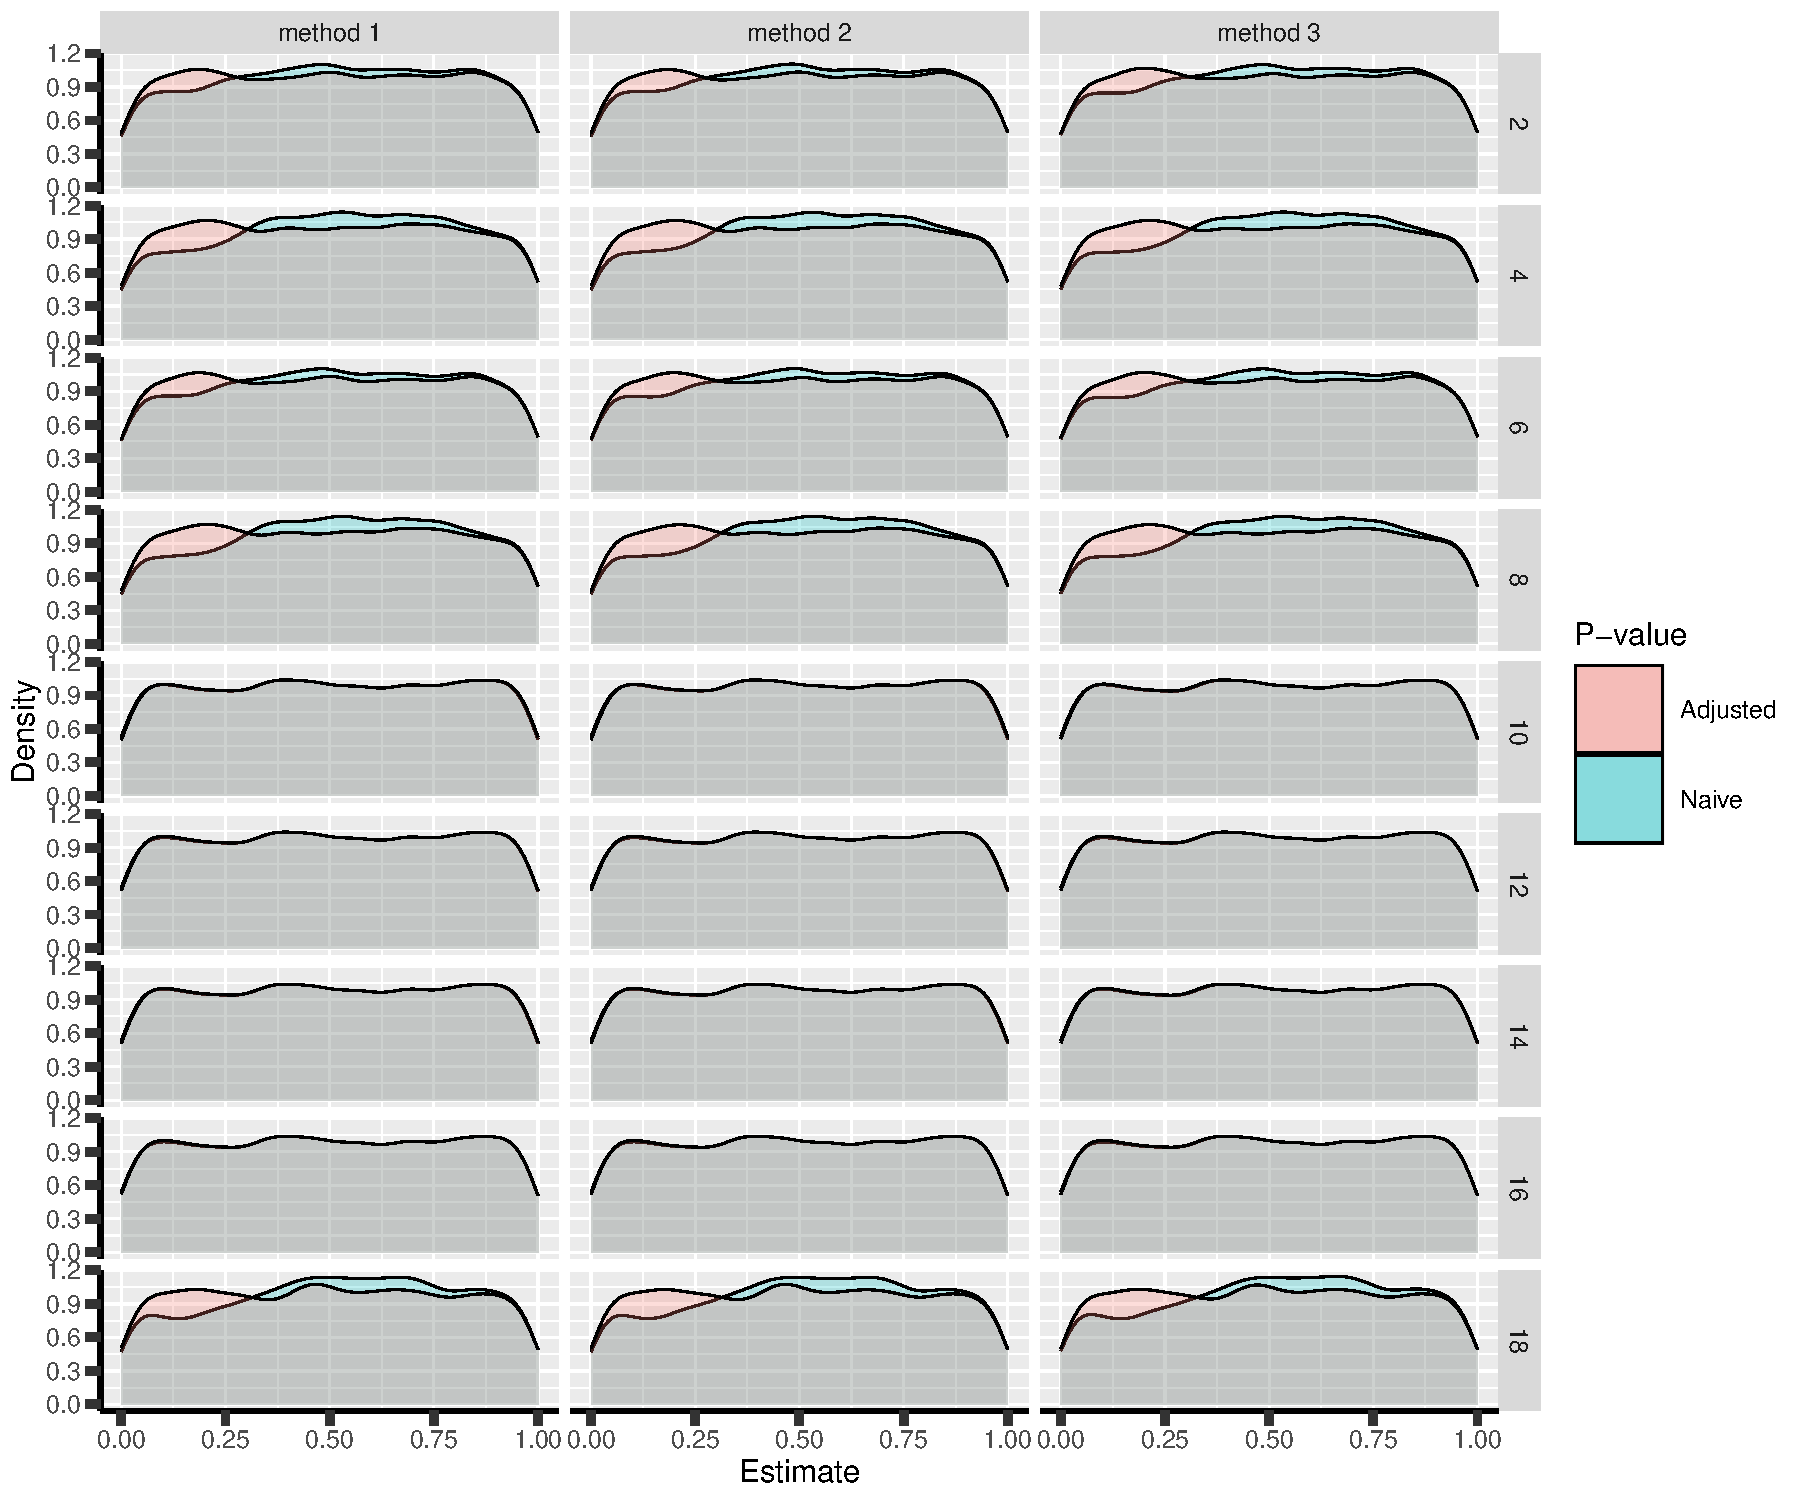
\includegraphics[trim={0 0 0 0},width=1\textwidth]{./figures/gg2stage-pvalue-density.pdf}
\caption{Naive and adjusted p-value distribution over all simulations under the null. Each row correspond to a different scenario}
\end{figure}

\begin{figure}[!h]
\centering
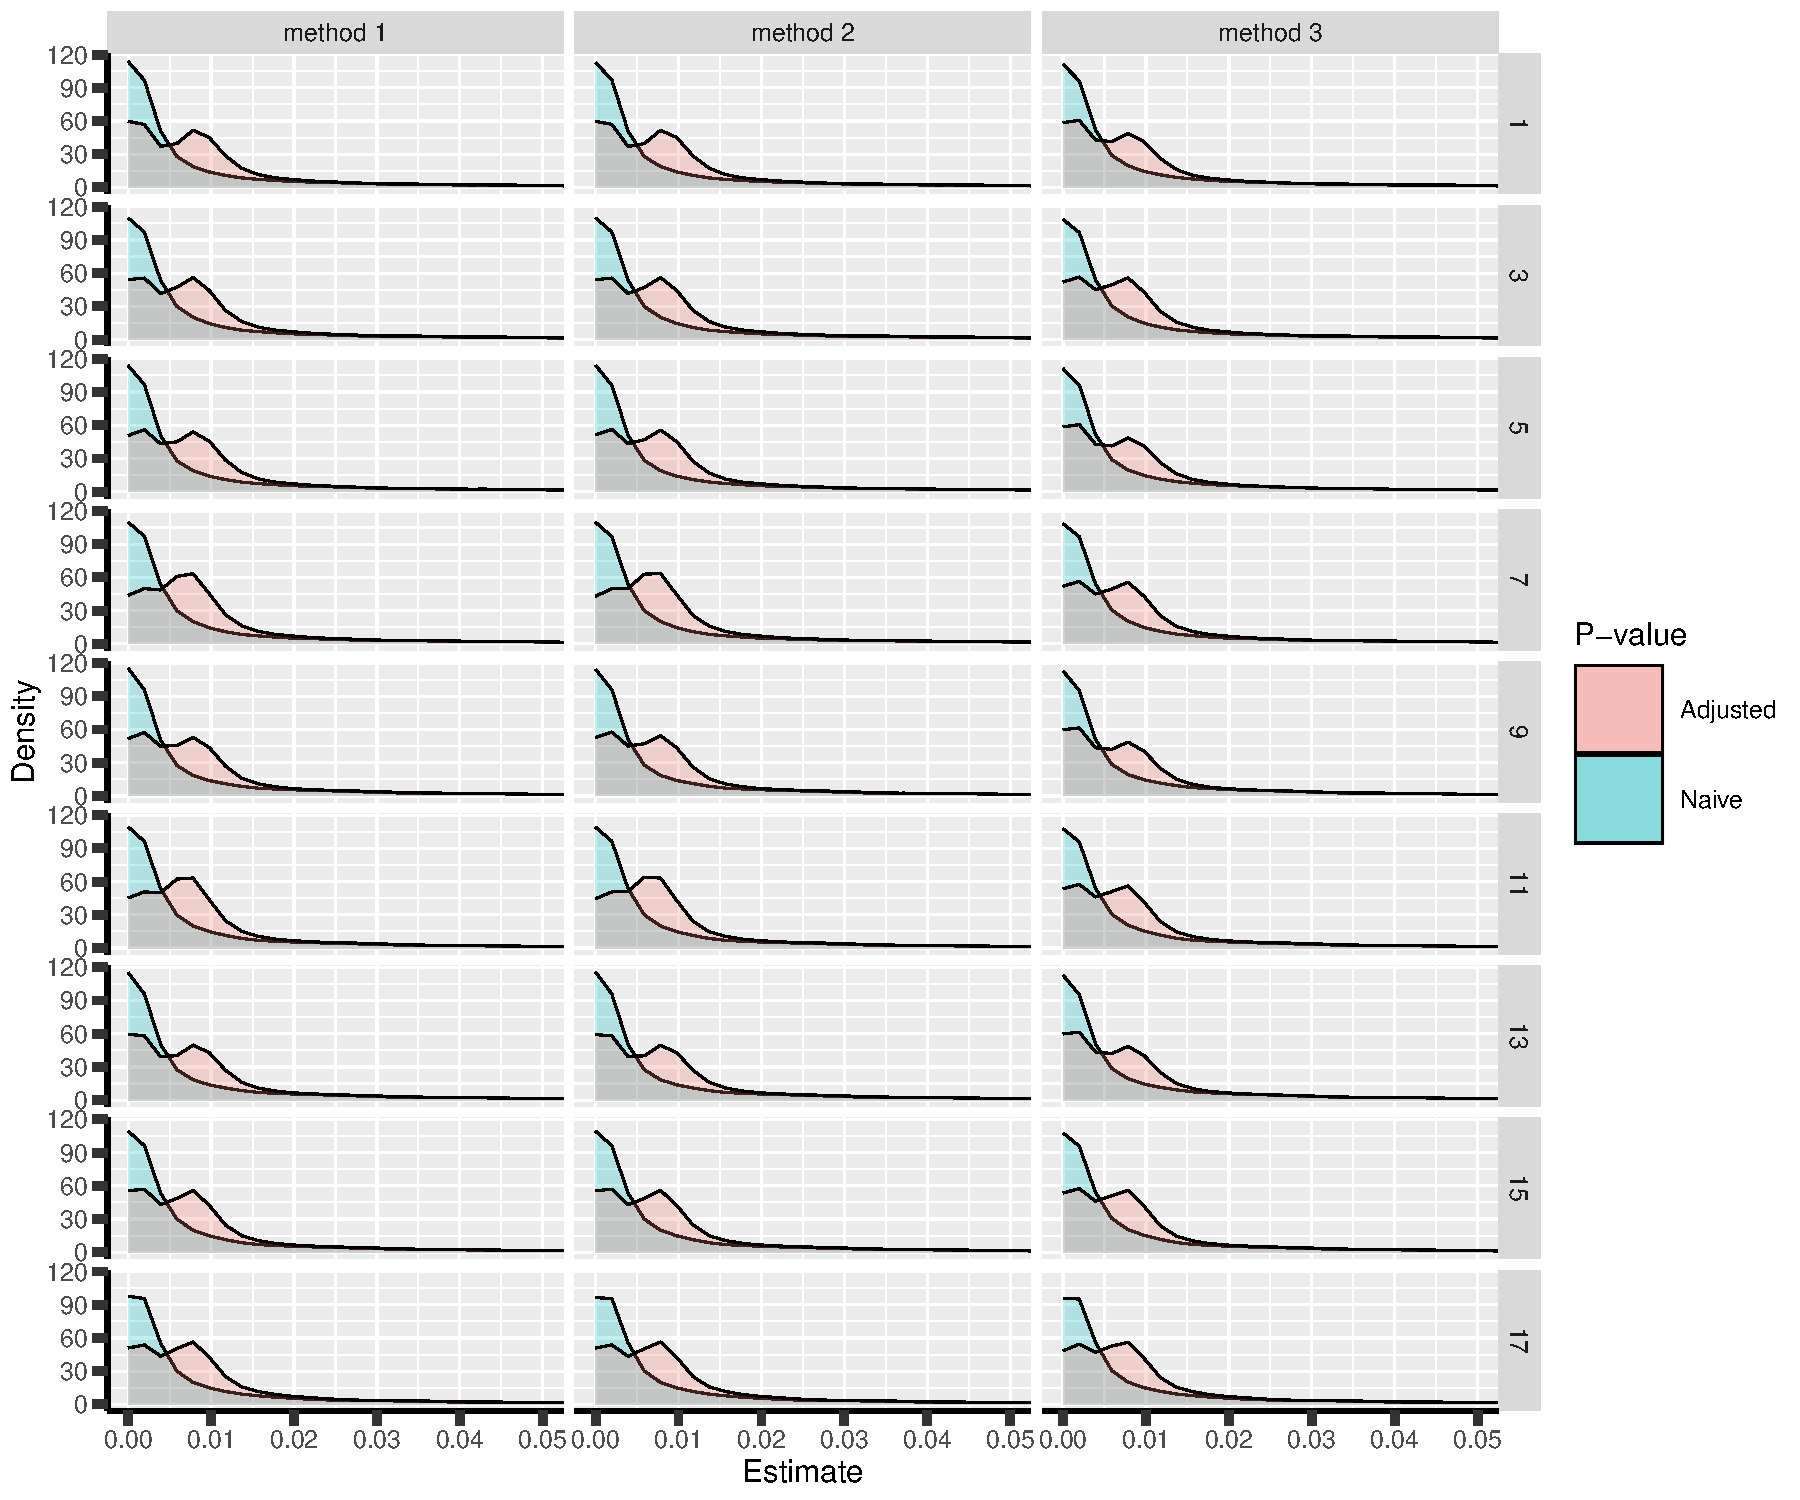
\includegraphics[trim={0 0 0 0},width=1\textwidth]{./figures/gg2stage-pvalue2-density.pdf}
\caption{Naive and adjusted p-value distribution over all simulations under the alternative. Each row correspond to a different scenario}
\end{figure}

\clearpage

\subsection{3 stages}
\label{sec:org7c6c38a}
Power by method (columns) and scenario (rows): \hfill (nominal level 80\%)
\begin{verbatim}
scenario n.sim missing binding  fixC ar method 1 method 2 method 3
       1  1868    TRUE    TRUE FALSE 10   75.32%   75.32%   75.00%
       5  1934    TRUE    TRUE  TRUE 10   75.18%   76.01%   76.11%
       7   245    TRUE    TRUE  TRUE  5   75.51%   75.92%   75.92%
       9  2500    TRUE   FALSE  TRUE 10   74.80%   75.32%   75.00%
      11  2500    TRUE   FALSE  TRUE  5   74.76%   75.44%   74.68%
      13  2500    TRUE   FALSE FALSE 10   75.28%   75.40%   75.36%
      15  2500    TRUE   FALSE FALSE  5   75.12%   75.24%   75.12%
\end{verbatim}


\bigskip

Type 1 error by method (columns) and scenario (rows): \hfill (nominal level 2.5\%)
\begin{verbatim}
scenario n.sim missing binding  fixC ar method 1 method 2 method 3
       2  2481    TRUE    TRUE FALSE 10    2.94%    2.94%    2.70%
       4  1127    TRUE    TRUE FALSE  5    3.11%    3.11%    3.11%
       6  2432    TRUE    TRUE  TRUE 10    1.89%    2.14%    2.01%
       8  1042    TRUE    TRUE  TRUE  5    1.73%    1.92%    1.82%
      10  2500    TRUE   FALSE  TRUE 10    2.36%    2.40%    2.32%
      12  2500    TRUE   FALSE  TRUE  5    2.36%    2.28%    2.28%
      14  2483    TRUE   FALSE FALSE 10    3.02%    3.10%    3.10%
      16  2500    TRUE   FALSE FALSE  5    3.16%    3.12%    3.04%
\end{verbatim}


\clearpage

\begin{figure}[!h]
\centering
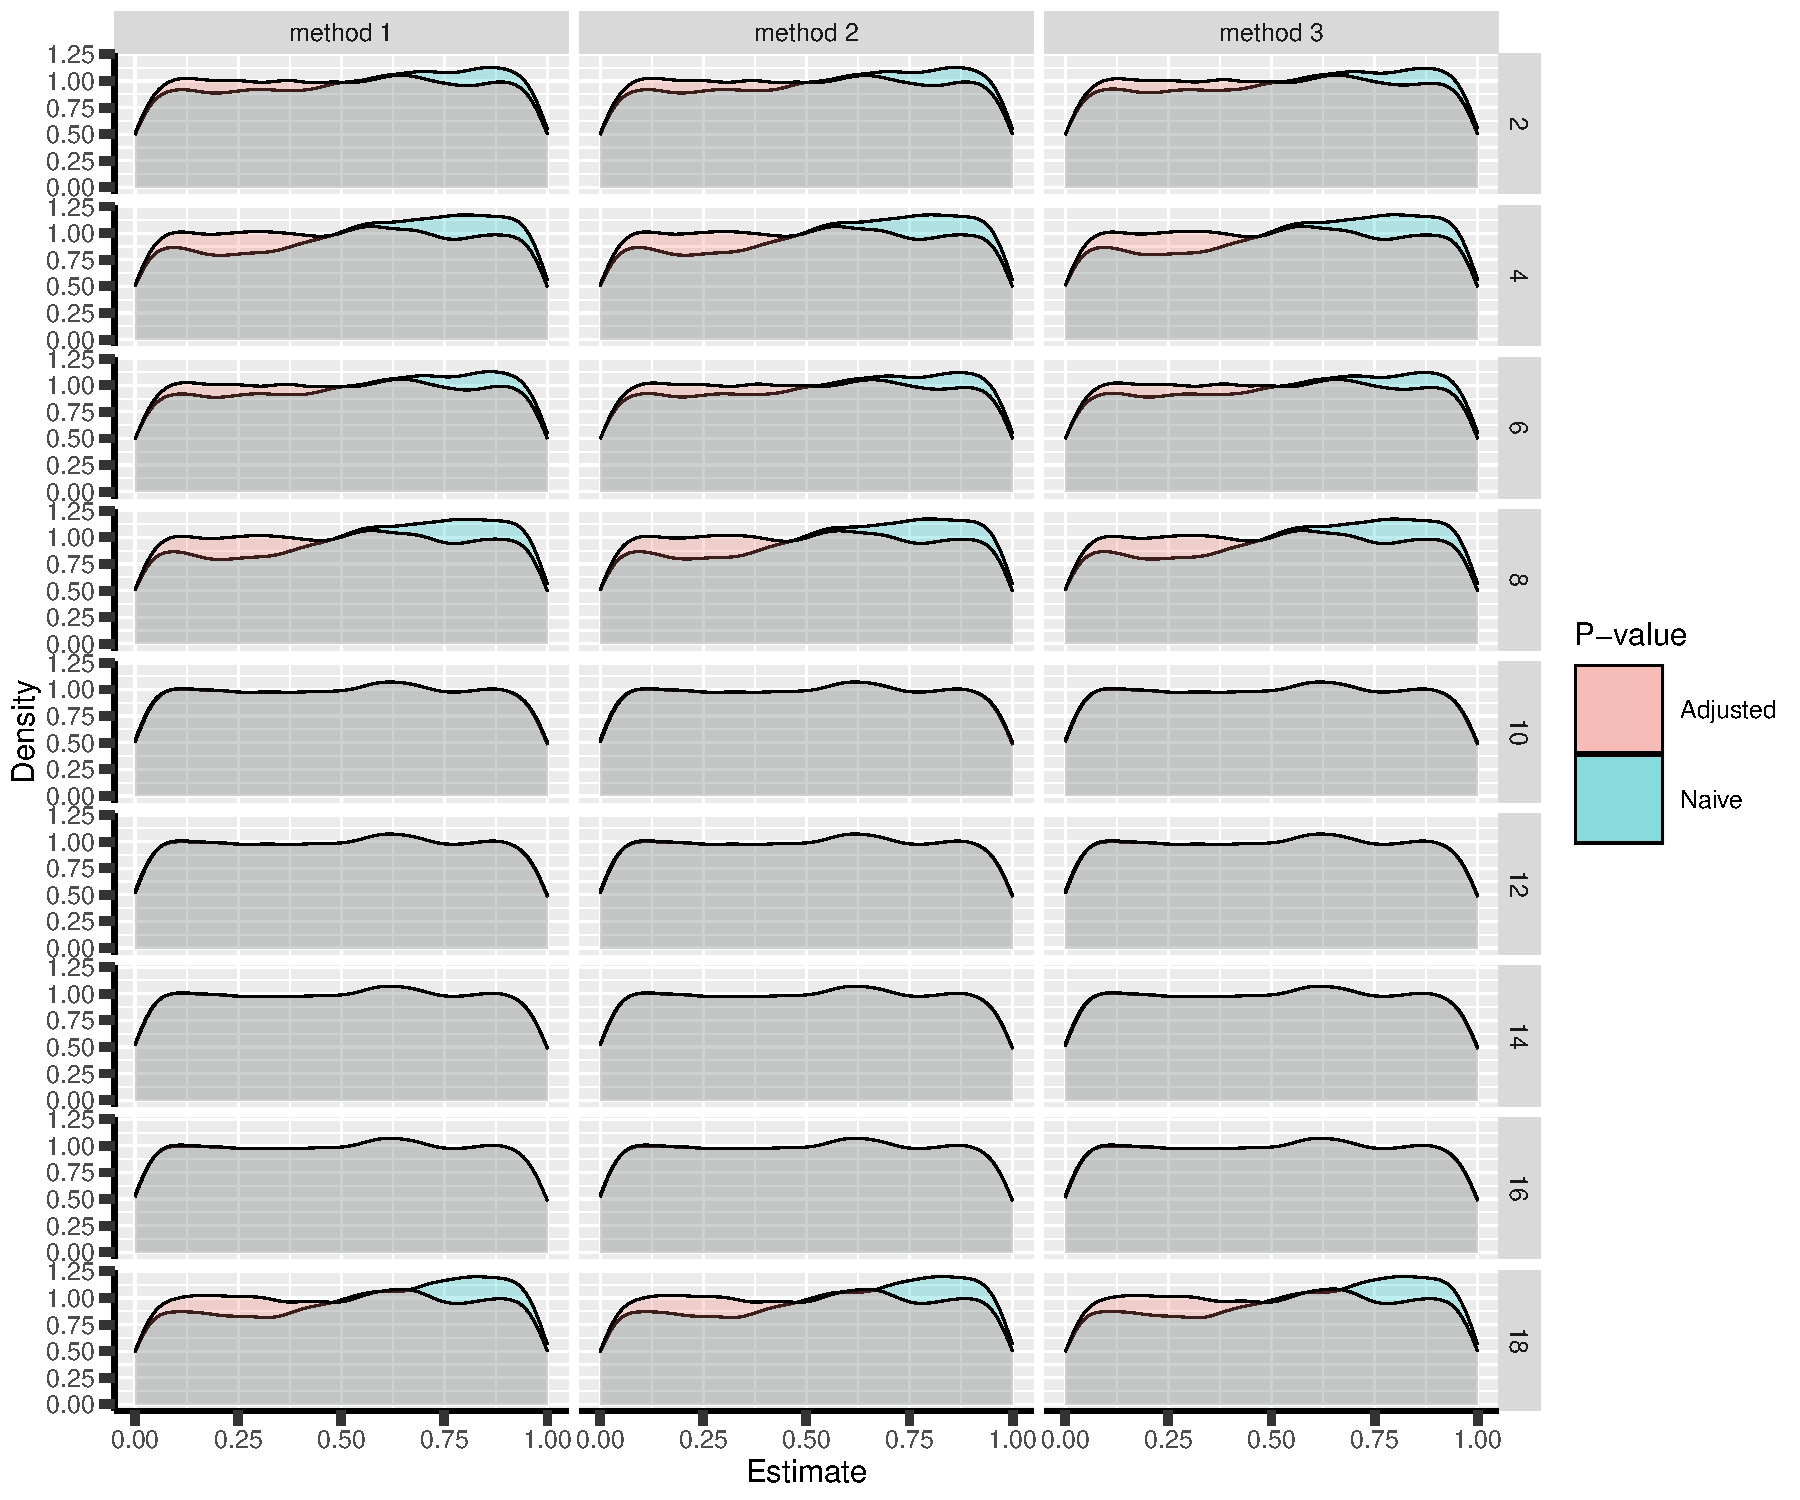
\includegraphics[trim={0 0 0 0},width=1\textwidth]{./figures/gg3stage-pvalue-density.pdf}
\caption{Naive and adjusted p-value distribution over all simulations under the null. Each row correspond to a different scenario}
\end{figure}

\begin{figure}[!h]
\centering
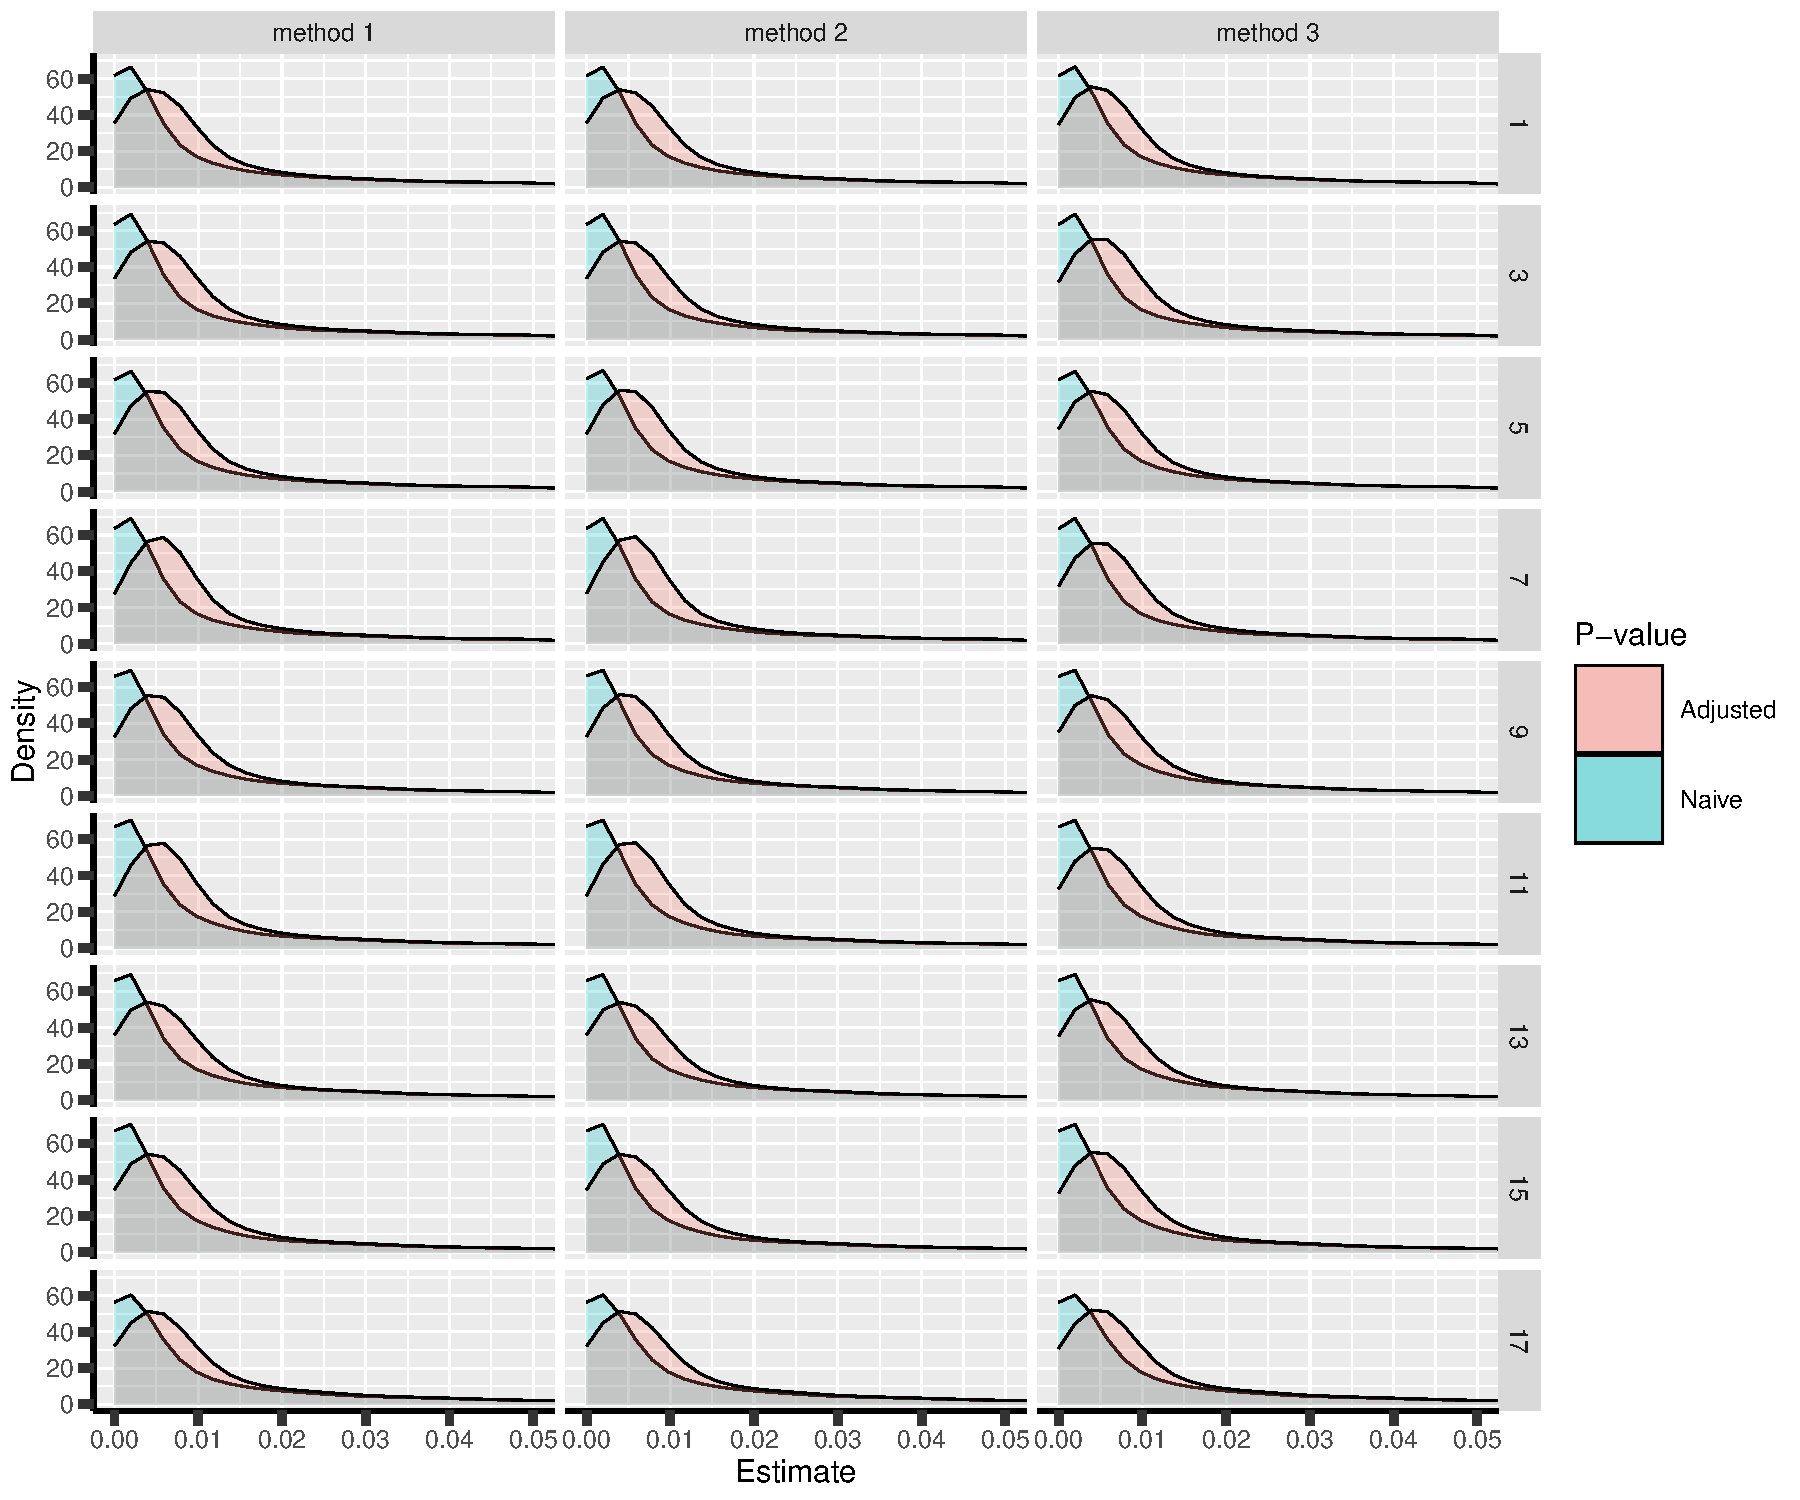
\includegraphics[trim={0 0 0 0},width=1\textwidth]{./figures/gg-pvalue2-density.pdf}
\caption{Naive and adjusted p-value distribution over all simulations under the alternative. Each row correspond to a different scenario}
\end{figure}

\clearpage

\section{Conclusion of the trial}
\label{sec:orga165221}

\subsection{2 stages}
\label{sec:org771dea9}
Relative frequency of stopping for efficacy/futility at decision/final

\begin{itemize}
\item Method 1
\end{itemize}
\begin{verbatim}
        N missing  hypo binding  fixC ar decision.eff decision.fut final.eff final.fut
 1: 10000    TRUE power    TRUE FALSE 10       37.79%        5.93%    43.21%    13.07%
 2: 10000    TRUE typeI    TRUE FALSE 10        0.80%       71.13%     1.62%    26.45%
 3: 10000    TRUE power    TRUE FALSE  5       35.74%        5.98%    44.79%    13.49%
 4: 10000    TRUE typeI    TRUE FALSE  5        0.74%       69.32%     1.66%    28.28%
 5: 10000    TRUE power    TRUE  TRUE 10       36.94%        6.78%    43.21%    13.07%
 6: 10000    TRUE typeI    TRUE  TRUE 10        0.62%       71.31%     1.62%    26.45%
 7: 10000    TRUE power    TRUE  TRUE  5       35.29%        6.43%    44.79%    13.49%
 8: 10000    TRUE typeI    TRUE  TRUE  5        0.66%       69.40%     1.66%    28.28%
 9: 10000    TRUE power   FALSE  TRUE 10       38.05%        6.57%    41.81%    13.57%
10: 10000    TRUE typeI   FALSE  TRUE 10        0.61%        0.20%     1.84%    97.35%
11: 10000    TRUE power   FALSE  TRUE  5       36.35%        6.15%    43.58%    13.92%
12: 10000    TRUE typeI   FALSE  TRUE  5        0.70%        0.06%     1.93%    97.31%
13: 10000    TRUE power   FALSE FALSE 10       38.69%        5.93%    41.81%    13.57%
14: 10000    TRUE typeI   FALSE FALSE 10        0.69%        0.12%     1.84%    97.35%
15: 10000    TRUE power   FALSE FALSE  5       36.79%        5.71%    43.58%    13.92%
16: 10000    TRUE typeI   FALSE FALSE  5        0.75%        0.01%     1.93%    97.31%
17: 10000   FALSE power    TRUE FALSE  5       33.98%        5.33%    46.33%    14.36%
18: 10000   FALSE typeI    TRUE FALSE  5        0.74%       67.48%     1.72%    30.06%
\end{verbatim}

\clearpage

Method 2:
\begin{verbatim}
        N missing  hypo binding  fixC ar decision.eff decision.fut final.eff final.fut
 1: 10000    TRUE power    TRUE FALSE 10       37.85%        6.19%    43.08%    12.88%
 2: 10000    TRUE typeI    TRUE FALSE 10        0.79%       71.64%     1.60%    25.97%
 3: 10000    TRUE power    TRUE FALSE  5       35.77%        5.99%    44.76%    13.48%
 4: 10000    TRUE typeI    TRUE FALSE  5        0.74%       69.38%     1.66%    28.22%
 5: 10000    TRUE power    TRUE  TRUE 10       36.69%        6.24%    43.66%    13.41%
 6: 10000    TRUE typeI    TRUE  TRUE 10        0.59%       69.61%     1.63%    28.17%
 7: 10000    TRUE power    TRUE  TRUE  5       35.02%        6.05%    45.18%    13.75%
 8: 10000    TRUE typeI    TRUE  TRUE  5        0.63%       68.36%     1.68%    29.33%
 9: 10000    TRUE power   FALSE  TRUE 10       37.85%        6.04%    42.27%    13.84%
10: 10000    TRUE typeI   FALSE  TRUE 10        0.61%        0.19%     1.86%    97.34%
11: 10000    TRUE power   FALSE  TRUE  5       36.18%        5.84%    43.86%    14.12%
12: 10000    TRUE typeI   FALSE  TRUE  5        0.69%        0.06%     1.95%    97.30%
13: 10000    TRUE power   FALSE FALSE 10       38.70%        6.09%    41.74%    13.47%
14: 10000    TRUE typeI   FALSE FALSE 10        0.69%        0.12%     1.84%    97.35%
15: 10000    TRUE power   FALSE FALSE  5       36.82%        5.75%    43.54%    13.89%
16: 10000    TRUE typeI   FALSE FALSE  5        0.75%        0.01%     1.93%    97.31%
17: 10000   FALSE power    TRUE FALSE  5       34.03%        5.36%    46.27%    14.34%
18: 10000   FALSE typeI    TRUE FALSE  5        0.74%       67.55%     1.72%    29.99%
\end{verbatim}

Method 3:
\begin{verbatim}
        N missing  hypo binding  fixC ar decision.eff decision.fut final.eff final.fut
 1: 10000    TRUE power    TRUE FALSE 10       40.58%        6.53%    39.85%    13.04%
 2: 10000    TRUE typeI    TRUE FALSE 10        0.74%       68.79%     1.63%    28.84%
 3: 10000    TRUE power    TRUE FALSE  5       36.54%        6.30%    43.60%    13.56%
 4: 10000    TRUE typeI    TRUE FALSE  5        0.69%       68.41%     1.66%    29.24%
 5: 10000    TRUE power    TRUE  TRUE 10       40.58%        6.53%    39.85%    13.04%
 6: 10000    TRUE typeI    TRUE  TRUE 10        0.74%       68.79%     1.63%    28.84%
 7: 10000    TRUE power    TRUE  TRUE  5       36.54%        6.30%    43.60%    13.56%
 8: 10000    TRUE typeI    TRUE  TRUE  5        0.69%       68.41%     1.66%    29.24%
 9: 10000    TRUE power   FALSE  TRUE 10       41.34%        6.20%    38.92%    13.54%
10: 10000    TRUE typeI   FALSE  TRUE 10        0.77%        0.33%     1.80%    97.10%
11: 10000    TRUE power   FALSE  TRUE  5       37.71%        6.03%    42.35%    13.91%
12: 10000    TRUE typeI   FALSE  TRUE  5        0.73%        0.09%     1.93%    97.25%
13: 10000    TRUE power   FALSE FALSE 10       41.34%        6.20%    38.92%    13.54%
14: 10000    TRUE typeI   FALSE FALSE 10        0.77%        0.33%     1.80%    97.10%
15: 10000    TRUE power   FALSE FALSE  5       37.71%        6.03%    42.35%    13.91%
16: 10000    TRUE typeI   FALSE FALSE  5        0.73%        0.09%     1.93%    97.25%
17: 10000   FALSE power    TRUE FALSE  5       34.65%        5.59%    45.27%    14.49%
18: 10000   FALSE typeI    TRUE FALSE  5        0.68%       66.54%     1.77%    31.01%
\end{verbatim}

\clearpage

Relative frequency of stopping for with a threshold below 1.96:
\begin{verbatim}
    scenario missing method binding  fixC ar  hypo     N rejection rejectionBelow196
 1:        1    TRUE      1    TRUE FALSE 10 power 10000    81.00%             0.85%
 2:        1    TRUE      2    TRUE FALSE 10 power 10000    80.93%             0.84%
 3:        2    TRUE      1    TRUE FALSE 10 typeI 10000     2.42%             0.18%
 4:        2    TRUE      2    TRUE FALSE 10 typeI 10000     2.39%             0.17%
 5:        3    TRUE      1    TRUE FALSE  5 power 10000    80.53%             0.45%
 6:        3    TRUE      2    TRUE FALSE  5 power 10000    80.53%             0.45%
 7:        4    TRUE      1    TRUE FALSE  5 typeI 10000     2.40%             0.08%
 8:        4    TRUE      2    TRUE FALSE  5 typeI 10000     2.40%             0.08%
 9:       13    TRUE      1   FALSE FALSE 10 power 10000    80.50%             0.64%
10:       13    TRUE      2   FALSE FALSE 10 power 10000    80.44%             0.64%
11:       14    TRUE      1   FALSE FALSE 10 typeI 10000     2.53%             0.08%
12:       14    TRUE      2   FALSE FALSE 10 typeI 10000     2.53%             0.08%
13:       15    TRUE      1   FALSE FALSE  5 power 10000    80.37%             0.44%
14:       15    TRUE      2   FALSE FALSE  5 power 10000    80.36%             0.44%
15:       16    TRUE      1   FALSE FALSE  5 typeI 10000     2.68%             0.05%
16:       16    TRUE      2   FALSE FALSE  5 typeI 10000     2.68%             0.05%
17:       17   FALSE      1    TRUE FALSE  5 power 10000    80.31%             0.42%
18:       17   FALSE      2    TRUE FALSE  5 power 10000    80.30%             0.43%
19:       18   FALSE      1    TRUE FALSE  5 typeI 10000     2.46%             0.08%
20:       18   FALSE      2    TRUE FALSE  5 typeI 10000     2.46%             0.08%
\end{verbatim}

\clearpage

\subsection{3 stages}
\label{sec:org5eaea5e}
Relative frequency of stopping for efficacy/futility at decision/final

\begin{itemize}
\item Method 1
\end{itemize}
\begin{verbatim}
       N missing  hypo binding  fixC ar dec1.eff dec1.fut dec2.eff dec2.fut final.eff final.fut
 1: 1868    TRUE power    TRUE FALSE 10    8.73%    1.93%   19.86%    3.37%    46.73%    19.38%
 2: 2481    TRUE typeI    TRUE FALSE 10    0.32%   26.64%    0.60%   35.95%     2.02%    34.46%
 3: 1127    TRUE typeI    TRUE FALSE  5    0.44%   30.26%    0.27%   36.11%     2.40%    30.52%
 4: 1934    TRUE power    TRUE  TRUE 10    9.31%    1.71%   19.65%    3.67%    46.23%    19.44%
 5: 2432    TRUE typeI    TRUE  TRUE 10    0.08%   25.82%    0.16%   36.06%     1.64%    36.23%
 6:  245    TRUE power    TRUE  TRUE  5   14.29%    2.04%   13.47%    6.12%    47.76%    16.33%
 7: 1042    TRUE typeI    TRUE  TRUE  5    0.19%   27.45%        0   37.04%     1.54%    33.78%
 8: 2500    TRUE power   FALSE  TRUE 10    9.84%    1.88%   21.20%    3.60%    43.76%    19.72%
 9: 2500    TRUE typeI   FALSE  TRUE 10    0.20%    0.04%    0.44%    0.12%     1.72%    97.48%
10: 2500    TRUE power   FALSE  TRUE  5   10.32%    1.80%   21.04%    3.32%    43.40%    20.12%
11: 2500    TRUE typeI   FALSE  TRUE  5    0.08%    0.04%    0.52%        0     1.76%    97.60%
12: 2500    TRUE power   FALSE FALSE 10    9.36%    1.48%   20.68%    3.56%    45.24%    19.68%
13: 2483    TRUE typeI   FALSE FALSE 10    0.36%    0.12%    0.20%    0.04%     2.46%    96.82%
14: 2500    TRUE power   FALSE FALSE  5    9.92%    1.80%   20.64%    3.56%    44.56%    19.52%
15: 2500    TRUE typeI   FALSE FALSE  5    0.44%        0    0.40%        0     2.32%    96.84%
\end{verbatim}

\begin{itemize}
\item Method 2
\end{itemize}
\begin{verbatim}
       N missing  hypo binding  fixC ar dec1.eff dec1.fut dec2.eff dec2.fut final.eff final.fut
 1: 1868    TRUE power    TRUE FALSE 10    8.73%    1.93%   19.86%    3.37%    46.73%    19.38%
 2: 2481    TRUE typeI    TRUE FALSE 10    0.32%   26.68%    0.60%   35.99%     2.02%    34.38%
 3: 1127    TRUE typeI    TRUE FALSE  5    0.44%   30.35%    0.27%   36.02%     2.40%    30.52%
 4: 1934    TRUE power    TRUE  TRUE 10    9.46%    1.60%   20.42%    3.41%    46.12%    18.98%
 5: 2432    TRUE typeI    TRUE  TRUE 10    0.12%   24.96%    0.16%   35.44%     1.85%    37.46%
 6:  245    TRUE power    TRUE  TRUE  5   13.88%    2.04%   13.06%    6.53%    48.98%    15.51%
 7: 1042    TRUE typeI    TRUE  TRUE  5    0.19%   26.97%    0.10%   37.04%     1.63%    34.07%
 8: 2500    TRUE power   FALSE  TRUE 10    9.92%    1.76%   21.44%    3.40%    43.96%    19.52%
 9: 2500    TRUE typeI   FALSE  TRUE 10    0.24%    0.04%    0.44%    0.08%     1.72%    97.48%
10: 2500    TRUE power   FALSE  TRUE  5   10.36%    2.00%   21.32%    3.04%    43.76%    19.52%
11: 2500    TRUE typeI   FALSE  TRUE  5    0.08%    0.08%    0.52%        0     1.68%    97.64%
12: 2500    TRUE power   FALSE FALSE 10    9.36%    1.48%   20.72%    3.44%    45.32%    19.68%
13: 2483    TRUE typeI   FALSE FALSE 10    0.36%    0.12%    0.20%        0     2.54%    96.78%
14: 2500    TRUE power   FALSE FALSE  5    9.92%    1.80%   20.40%    3.28%    44.92%    19.68%
15: 2500    TRUE typeI   FALSE FALSE  5    0.44%        0    0.32%        0     2.36%    96.88%
\end{verbatim}

\clearpage

\begin{itemize}
\item Method 3
\end{itemize}
\begin{verbatim}
       N missing  hypo binding  fixC ar dec1.eff dec1.fut dec2.eff dec2.fut final.eff final.fut
 1: 1868    TRUE power    TRUE FALSE 10    8.94%    2.19%   20.77%    3.43%    45.29%    19.38%
 2: 2481    TRUE typeI    TRUE FALSE 10    0.24%   25.39%    0.48%   35.99%     1.98%    35.91%
 3: 1127    TRUE typeI    TRUE FALSE  5    0.35%   30.08%    0.27%   35.67%     2.48%    31.14%
 4: 1934    TRUE power    TRUE  TRUE 10    9.82%    1.55%   21.15%    3.46%    45.14%    18.87%
 5: 2432    TRUE typeI    TRUE  TRUE 10    0.08%   24.71%    0.21%   35.57%     1.73%    37.71%
 6:  245    TRUE power    TRUE  TRUE  5   14.69%    2.04%   13.88%    6.12%    47.35%    15.92%
 7: 1042    TRUE typeI    TRUE  TRUE  5    0.19%   27.06%        0   37.04%     1.63%    34.07%
 8: 2500    TRUE power   FALSE  TRUE 10   10.40%    1.80%   21.80%    3.32%    42.80%    19.88%
 9: 2500    TRUE typeI   FALSE  TRUE 10    0.20%    0.04%    0.44%    0.16%     1.68%    97.48%
10: 2500    TRUE power   FALSE  TRUE  5   10.64%    1.80%   21.04%    3.36%    43.00%    20.16%
11: 2500    TRUE typeI   FALSE  TRUE  5    0.12%    0.04%    0.48%        0     1.68%    97.68%
12: 2500    TRUE power   FALSE FALSE 10   10.36%    1.68%   21.36%    3.48%    43.64%    19.48%
13: 2483    TRUE typeI   FALSE FALSE 10    0.32%    0.16%    0.20%    0.04%     2.58%    96.70%
14: 2500    TRUE power   FALSE FALSE  5    9.96%    1.84%   20.68%    3.20%    44.48%    19.84%
15: 2500    TRUE typeI   FALSE FALSE  5    0.44%    0.04%    0.32%    0.04%     2.28%    96.88%
\end{verbatim}

Relative frequency of stopping for with a threshold below 1.96:
\begin{verbatim}
    scenario missing method binding  fixC ar  hypo    N rejection rejectionBelow196
 1:        1    TRUE      1    TRUE FALSE 10 power 1868    75.32%             0.64%
 2:        1    TRUE      2    TRUE FALSE 10 power 1868    75.32%             0.64%
 3:        2    TRUE      1    TRUE FALSE 10 typeI 2481     2.94%             0.24%
 4:        2    TRUE      2    TRUE FALSE 10 typeI 2481     2.94%             0.24%
 5:        4    TRUE      1    TRUE FALSE  5 typeI 1127     3.11%             0.09%
 6:        4    TRUE      2    TRUE FALSE  5 typeI 1127     3.11%             0.09%
 7:       13    TRUE      1   FALSE FALSE 10 power 2500    75.28%             0.36%
 8:       13    TRUE      2   FALSE FALSE 10 power 2500    75.40%             0.32%
 9:       14    TRUE      1   FALSE FALSE 10 typeI 2483     3.02%             0.04%
10:       14    TRUE      2   FALSE FALSE 10 typeI 2483     3.10%             0.04%
11:       15    TRUE      1   FALSE FALSE  5 power 2500    75.12%             0.16%
12:       15    TRUE      2   FALSE FALSE  5 power 2500    75.24%             0.16%
13:       16    TRUE      1   FALSE FALSE  5 typeI 2500     3.16%             0.08%
14:       16    TRUE      2   FALSE FALSE  5 typeI 2500     3.12%             0.08%
\end{verbatim}


\clearpage

\section{Bias (True effect: 0.6 under the alternative)}
\label{sec:org552c1f2}

\subsection{2 stages}
\label{sec:orgee86737}
Bias per estimator and method\footnote{e.g. \texttt{biasMLE1} mixed model
estimator (treatment effect), method 1 (boundaries)}:
\begin{adjustwidth}{-1cm}{-1cm}
\begin{verbatim}
     hypo missing binding  fixC ar biasMLE1 biasMLE2 biasMLE3 biasMUE1 biasMUE2 biasMUE3
 1: power    TRUE    TRUE FALSE 10  0.01345  0.01315  0.01468  0.00598  0.00566  0.00221
 2: typeI    TRUE    TRUE FALSE 10 -0.01794 -0.01784 -0.01856 -0.00453 -0.00448 -0.00510
 3: power    TRUE    TRUE FALSE  5  0.02257  0.02255  0.02358  0.01045  0.01048  0.00870
 4: typeI    TRUE    TRUE FALSE  5 -0.03034 -0.03031 -0.03065 -0.01190 -0.01185 -0.01243
 5: power    TRUE    TRUE  TRUE 10  0.01345  0.01403  0.01468  0.00110  0.00169  0.00221
 6: typeI    TRUE    TRUE  TRUE 10 -0.01794 -0.01871 -0.01856 -0.00542 -0.00609 -0.00510
 7: power    TRUE    TRUE  TRUE  5  0.02257  0.02309  0.02358  0.00788  0.00827  0.00870
 8: typeI    TRUE    TRUE  TRUE  5 -0.03034 -0.03085 -0.03065 -0.01230 -0.01288 -0.01243
 9: power    TRUE   FALSE  TRUE 10  0.01433  0.01490  0.01529  0.03456  0.03325  0.03453
10: typeI    TRUE   FALSE  TRUE 10  0.00019  0.00019  0.00051 -0.00076 -0.00068  0.00077
11: power    TRUE   FALSE  TRUE  5  0.02366  0.02402  0.02438  0.04130  0.04038  0.04201
12: typeI    TRUE   FALSE  TRUE  5  0.00091  0.00085  0.00101  0.00052  0.00047  0.00091
13: power    TRUE   FALSE FALSE 10  0.01433  0.01416  0.01529  0.03552  0.03589  0.03453
14: typeI    TRUE   FALSE FALSE 10  0.00019  0.00019  0.00051 -0.00020 -0.00021  0.00077
15: power    TRUE   FALSE FALSE  5  0.02366  0.02365  0.02438  0.04186  0.04202  0.04201
16: typeI    TRUE   FALSE FALSE  5  0.00091  0.00091  0.00101  0.00087  0.00087  0.00091
17: power   FALSE    TRUE FALSE  5  0.02284  0.02277  0.02381  0.01197  0.01196  0.01001
18: typeI   FALSE    TRUE FALSE  5 -0.02952 -0.02945 -0.02992 -0.01111 -0.01106 -0.01168
\end{verbatim}
\end{adjustwidth}

Median bias \footnote{Relative frequency at which the estimate is greater than the truth minus 0.5} per estimator and method:
\begin{adjustwidth}{-1cm}{-1cm}
\begin{verbatim}
     hypo missing binding  fixC ar mbiasMLE1 mbiasMLE2 mbiasMLE3 mbiasMUE1 mbiasMUE2 mbiasMUE3
 1: power    TRUE    TRUE FALSE 10    0.0261    0.0260    0.0301  -0.00240  -0.00250  -0.00535
 2: typeI    TRUE    TRUE FALSE 10   -0.0173   -0.0170   -0.0202   0.00100   0.00075  -0.00015
 3: power    TRUE    TRUE FALSE  5    0.0405    0.0405    0.0432  -0.00340  -0.00330  -0.00530
 4: typeI    TRUE    TRUE FALSE  5   -0.0330   -0.0329   -0.0345   0.00055   0.00055   0.00065
 5: power    TRUE    TRUE  TRUE 10    0.0261    0.0265    0.0301  -0.01050  -0.01010  -0.00535
 6: typeI    TRUE    TRUE  TRUE 10   -0.0173   -0.0197   -0.0202   0.00100  -0.00065  -0.00015
 7: power    TRUE    TRUE  TRUE  5    0.0405    0.0407    0.0432  -0.00770  -0.00650  -0.00530
 8: typeI    TRUE    TRUE  TRUE  5   -0.0330   -0.0346   -0.0345   0.00055   0.00075   0.00065
 9: power    TRUE   FALSE  TRUE 10    0.0326    0.0332    0.0327   0.02772   0.02517   0.02868
10: typeI    TRUE   FALSE  TRUE 10   -0.0009   -0.0009   -0.0009  -0.00190  -0.00185  -0.00025
11: power    TRUE   FALSE  TRUE  5    0.0462    0.0459    0.0489   0.02621   0.02512   0.02820
12: typeI    TRUE   FALSE  TRUE  5   -0.0009   -0.0010   -0.0009  -0.00130  -0.00140  -0.00015
13: power    TRUE   FALSE FALSE 10    0.0326    0.0324    0.0327   0.03094   0.03184   0.02868
14: typeI    TRUE   FALSE FALSE 10   -0.0009   -0.0009   -0.0009  -0.00150  -0.00140  -0.00025
15: power    TRUE   FALSE FALSE  5    0.0462    0.0464    0.0489   0.02832   0.02865   0.02820
16: typeI    TRUE   FALSE FALSE  5   -0.0009   -0.0009   -0.0009  -0.00105  -0.00105  -0.00015
17: power   FALSE    TRUE FALSE  5    0.0383    0.0383    0.0400  -0.00265  -0.00255  -0.00485
18: typeI   FALSE    TRUE FALSE  5   -0.0329   -0.0327   -0.0353   0.00420   0.00420   0.00330
\end{verbatim}

\end{adjustwidth}

\clearpage

\subsection{3 stages}
\label{sec:orgf87ffa6}
Bias per estimator and method\footnote{e.g. \texttt{biasMLE1} mixed model
estimator (treatment effect), method 1 (boundaries)}:
\begin{adjustwidth}{-1cm}{-1cm}
\begin{verbatim}
     hypo missing binding  fixC ar biasMLE1 biasMLE2 biasMLE3 biasMUE1 biasMUE2 biasMUE3
 1: power    TRUE    TRUE FALSE 10   0.0191   0.0191   0.0201   0.0181   0.0179   0.0133
 2: typeI    TRUE    TRUE FALSE 10  -0.0278  -0.0276  -0.0263  -0.0233  -0.0230  -0.0245
 3: typeI    TRUE    TRUE FALSE  5  -0.0688  -0.0690  -0.0693  -0.0528  -0.0531  -0.0541
 4: power    TRUE    TRUE  TRUE 10   0.0197   0.0202   0.0217   0.0187   0.0211   0.0200
 5: typeI    TRUE    TRUE  TRUE 10  -0.0341  -0.0336  -0.0340  -0.0252  -0.0240  -0.0253
 6: power    TRUE    TRUE  TRUE  5   0.0167   0.0148   0.0177   0.0354   0.0190   0.0157
 7: typeI    TRUE    TRUE  TRUE  5  -0.0547  -0.0539  -0.0542  -0.0342  -0.0350  -0.0361
 8: power    TRUE   FALSE  TRUE 10   0.0251   0.0254   0.0262   0.0561   0.0553   0.0523
 9: typeI    TRUE   FALSE  TRUE 10   0.0085   0.0081   0.0085   0.0100   0.0096   0.0101
10: power    TRUE   FALSE  TRUE  5   0.0377   0.0377   0.0374   0.0569   0.0570   0.0547
11: typeI    TRUE   FALSE  TRUE  5   0.0087   0.0085   0.0088   0.0092   0.0091   0.0092
12: power    TRUE   FALSE FALSE 10   0.0266   0.0268   0.0296   0.0539   0.0538   0.0536
13: typeI    TRUE   FALSE FALSE 10   0.0111   0.0106   0.0106   0.0130   0.0124   0.0130
14: power    TRUE   FALSE FALSE  5   0.0416   0.0419   0.0428   0.0605   0.0593   0.0584
15: typeI    TRUE   FALSE FALSE  5   0.0126   0.0122   0.0125   0.0137   0.0132   0.0134
\end{verbatim}
\end{adjustwidth}

Median bias \footnote{Relative frequency at which the estimate is greater than the truth minus 0.5} per estimator and method:
\begin{adjustwidth}{-1cm}{-1cm}
\begin{verbatim}
     hypo missing binding  fixC ar mbiasMLE1 mbiasMLE2 mbiasMLE3 mbiasMUE1 mbiasMUE2 mbiasMUE3
 1: power    TRUE    TRUE FALSE 10     0.034     0.034     0.038    0.0134    0.0134    0.0054
 2: typeI    TRUE    TRUE FALSE 10    -0.022    -0.022    -0.020    0.0147    0.0151    0.0139
 3: typeI    TRUE    TRUE FALSE  5    -0.072    -0.072    -0.075   -0.0138   -0.0129   -0.0138
 4: power    TRUE    TRUE  TRUE 10     0.028     0.029     0.029    0.0031    0.0041    0.0057
 5: typeI    TRUE    TRUE  TRUE 10    -0.029    -0.033    -0.032    0.0086    0.0095    0.0074
 6: power    TRUE    TRUE  TRUE  5    -0.018    -0.014    -0.018   -0.0347   -0.0347   -0.0429
 7: typeI    TRUE    TRUE  TRUE  5    -0.054    -0.047    -0.057   -0.0106   -0.0106   -0.0134
 8: power    TRUE   FALSE  TRUE 10     0.039     0.038     0.040    0.0520    0.0576    0.0484
 9: typeI    TRUE   FALSE  TRUE 10     0.022     0.023     0.020    0.0228    0.0232    0.0220
10: power    TRUE   FALSE  TRUE  5     0.048     0.050     0.046    0.0372    0.0428    0.0352
11: typeI    TRUE   FALSE  TRUE  5     0.023     0.023     0.021    0.0228    0.0236    0.0212
12: power    TRUE   FALSE FALSE 10     0.034     0.030     0.036    0.0460    0.0444    0.0408
13: typeI    TRUE   FALSE FALSE 10     0.018     0.015     0.015    0.0171    0.0151    0.0159
14: power    TRUE   FALSE FALSE  5     0.044     0.040     0.042    0.0452    0.0392    0.0384
15: typeI    TRUE   FALSE FALSE  5     0.018     0.015     0.015    0.0180    0.0152    0.0156
\end{verbatim}

\end{adjustwidth}

\clearpage

\section{Distribution of the estimates}
\label{sec:org1423ed4}

\subsection{2 stages}
\label{sec:org554815b}
Distribution of the estimates:
\begin{figure}[!h]
\centering
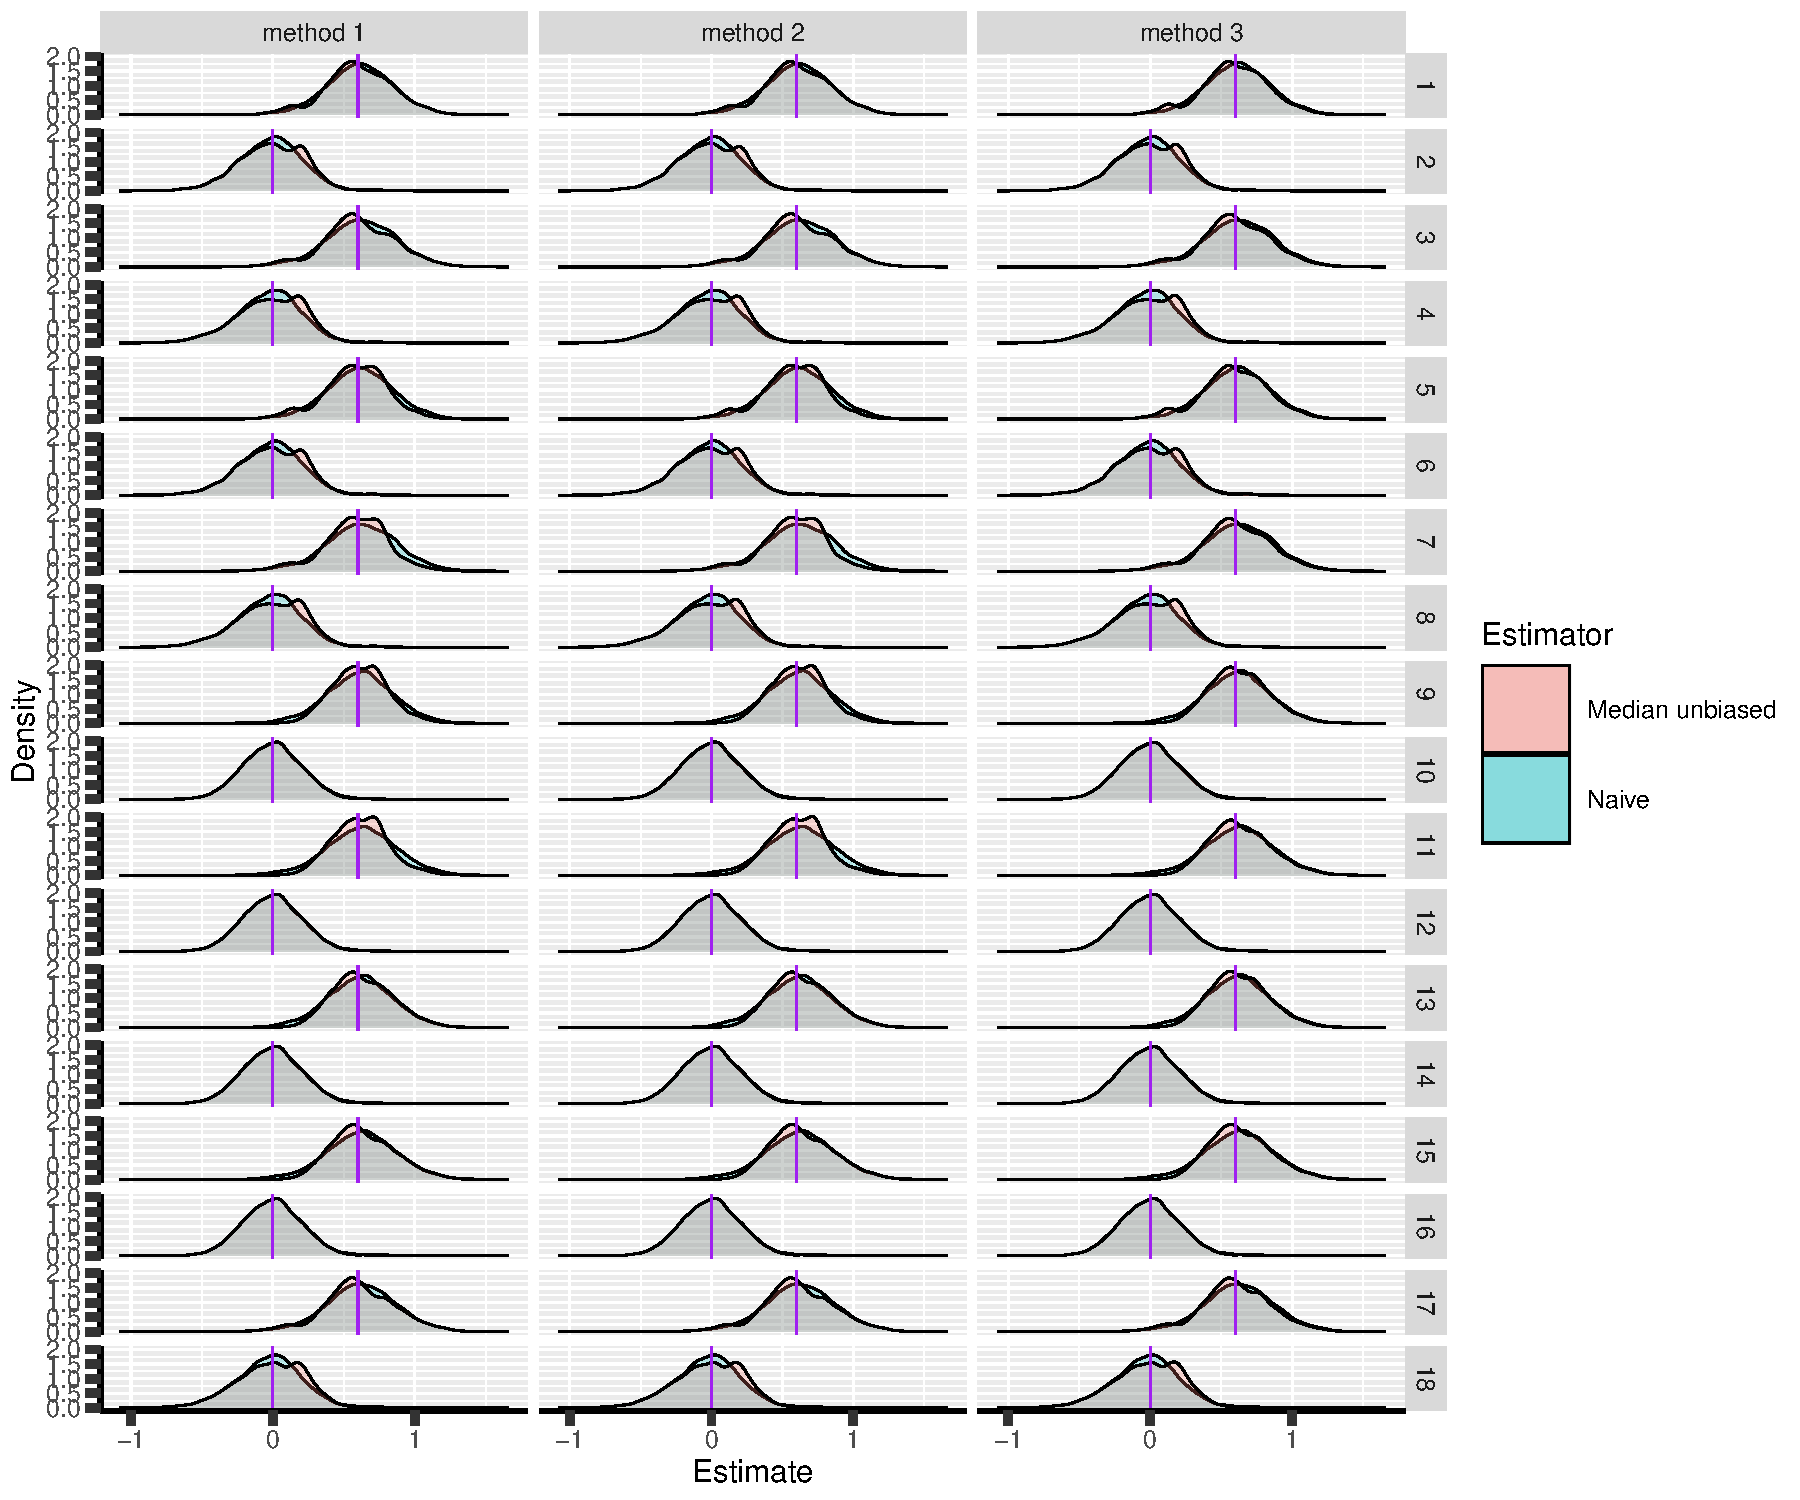
\includegraphics[trim={0 0 0 0},width=1\textwidth]{./figures/gg2stage-estimate-density.pdf}
\caption{Naive and Median unbiased estimate distribution over all simulations. Each row correspond to a different scenario}
\end{figure}

\begin{figure}[!h]
\centering
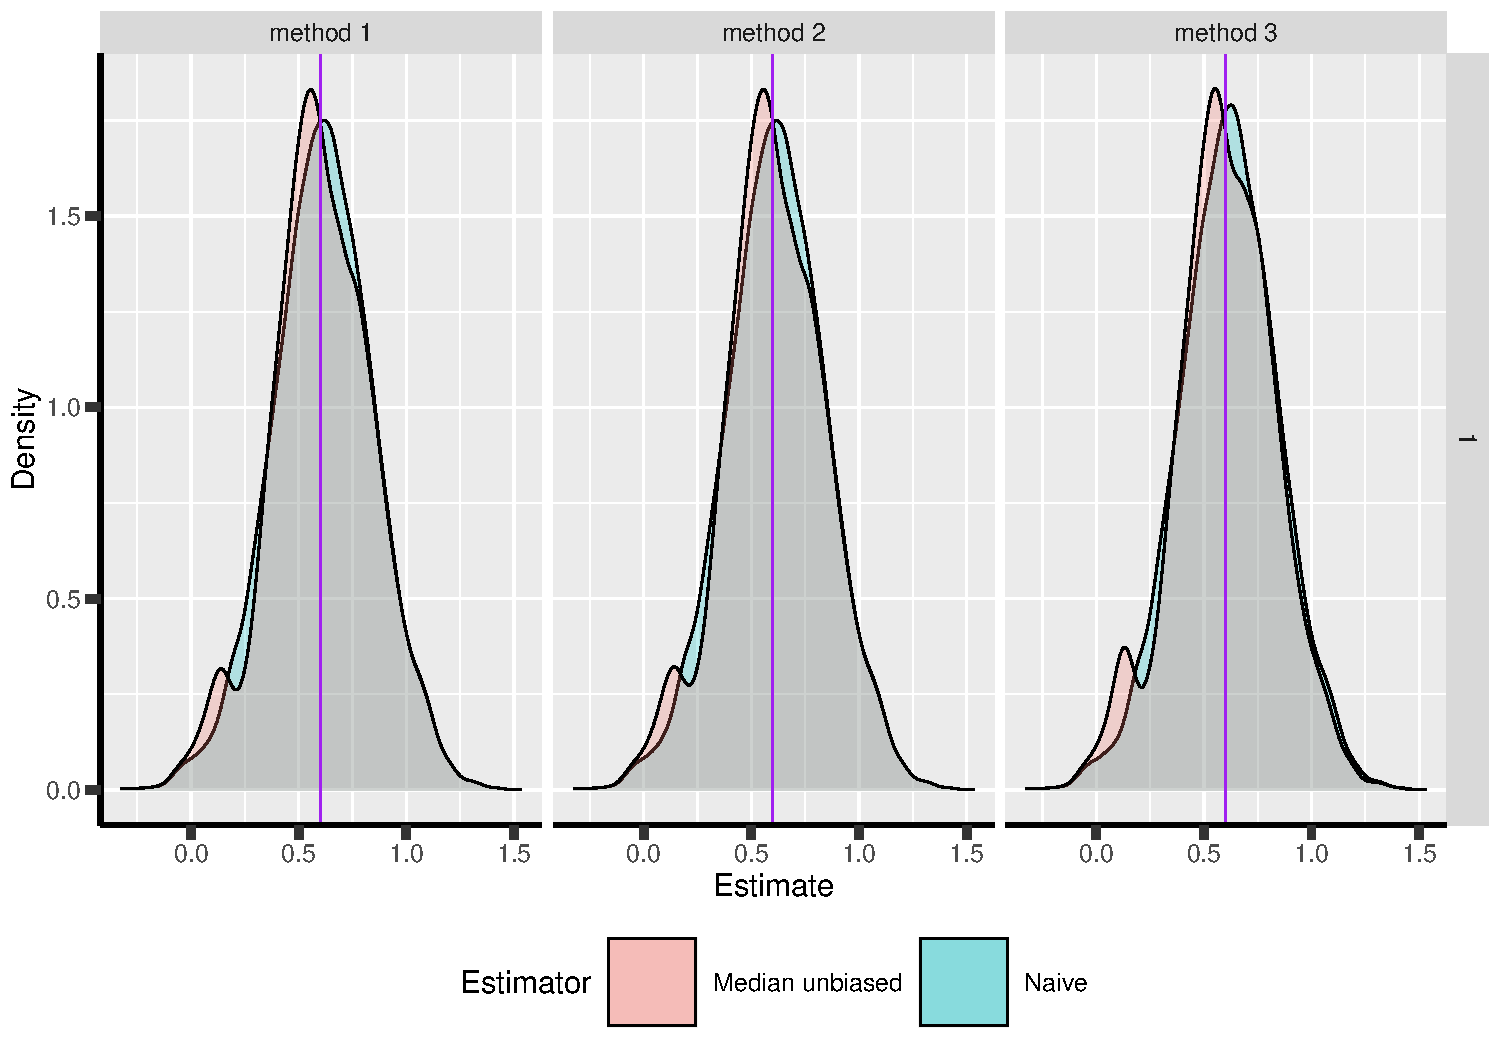
\includegraphics[trim={0 0 0 0},width=\textwidth]{./figures/gg2stage-estimate-density-scenario1.pdf}
\caption{Same but specific to scenario 1}
\end{figure}

\clearpage

Distribution of the median unbiased estimate conditional to the stage:
\begin{figure}[!h]
\centering
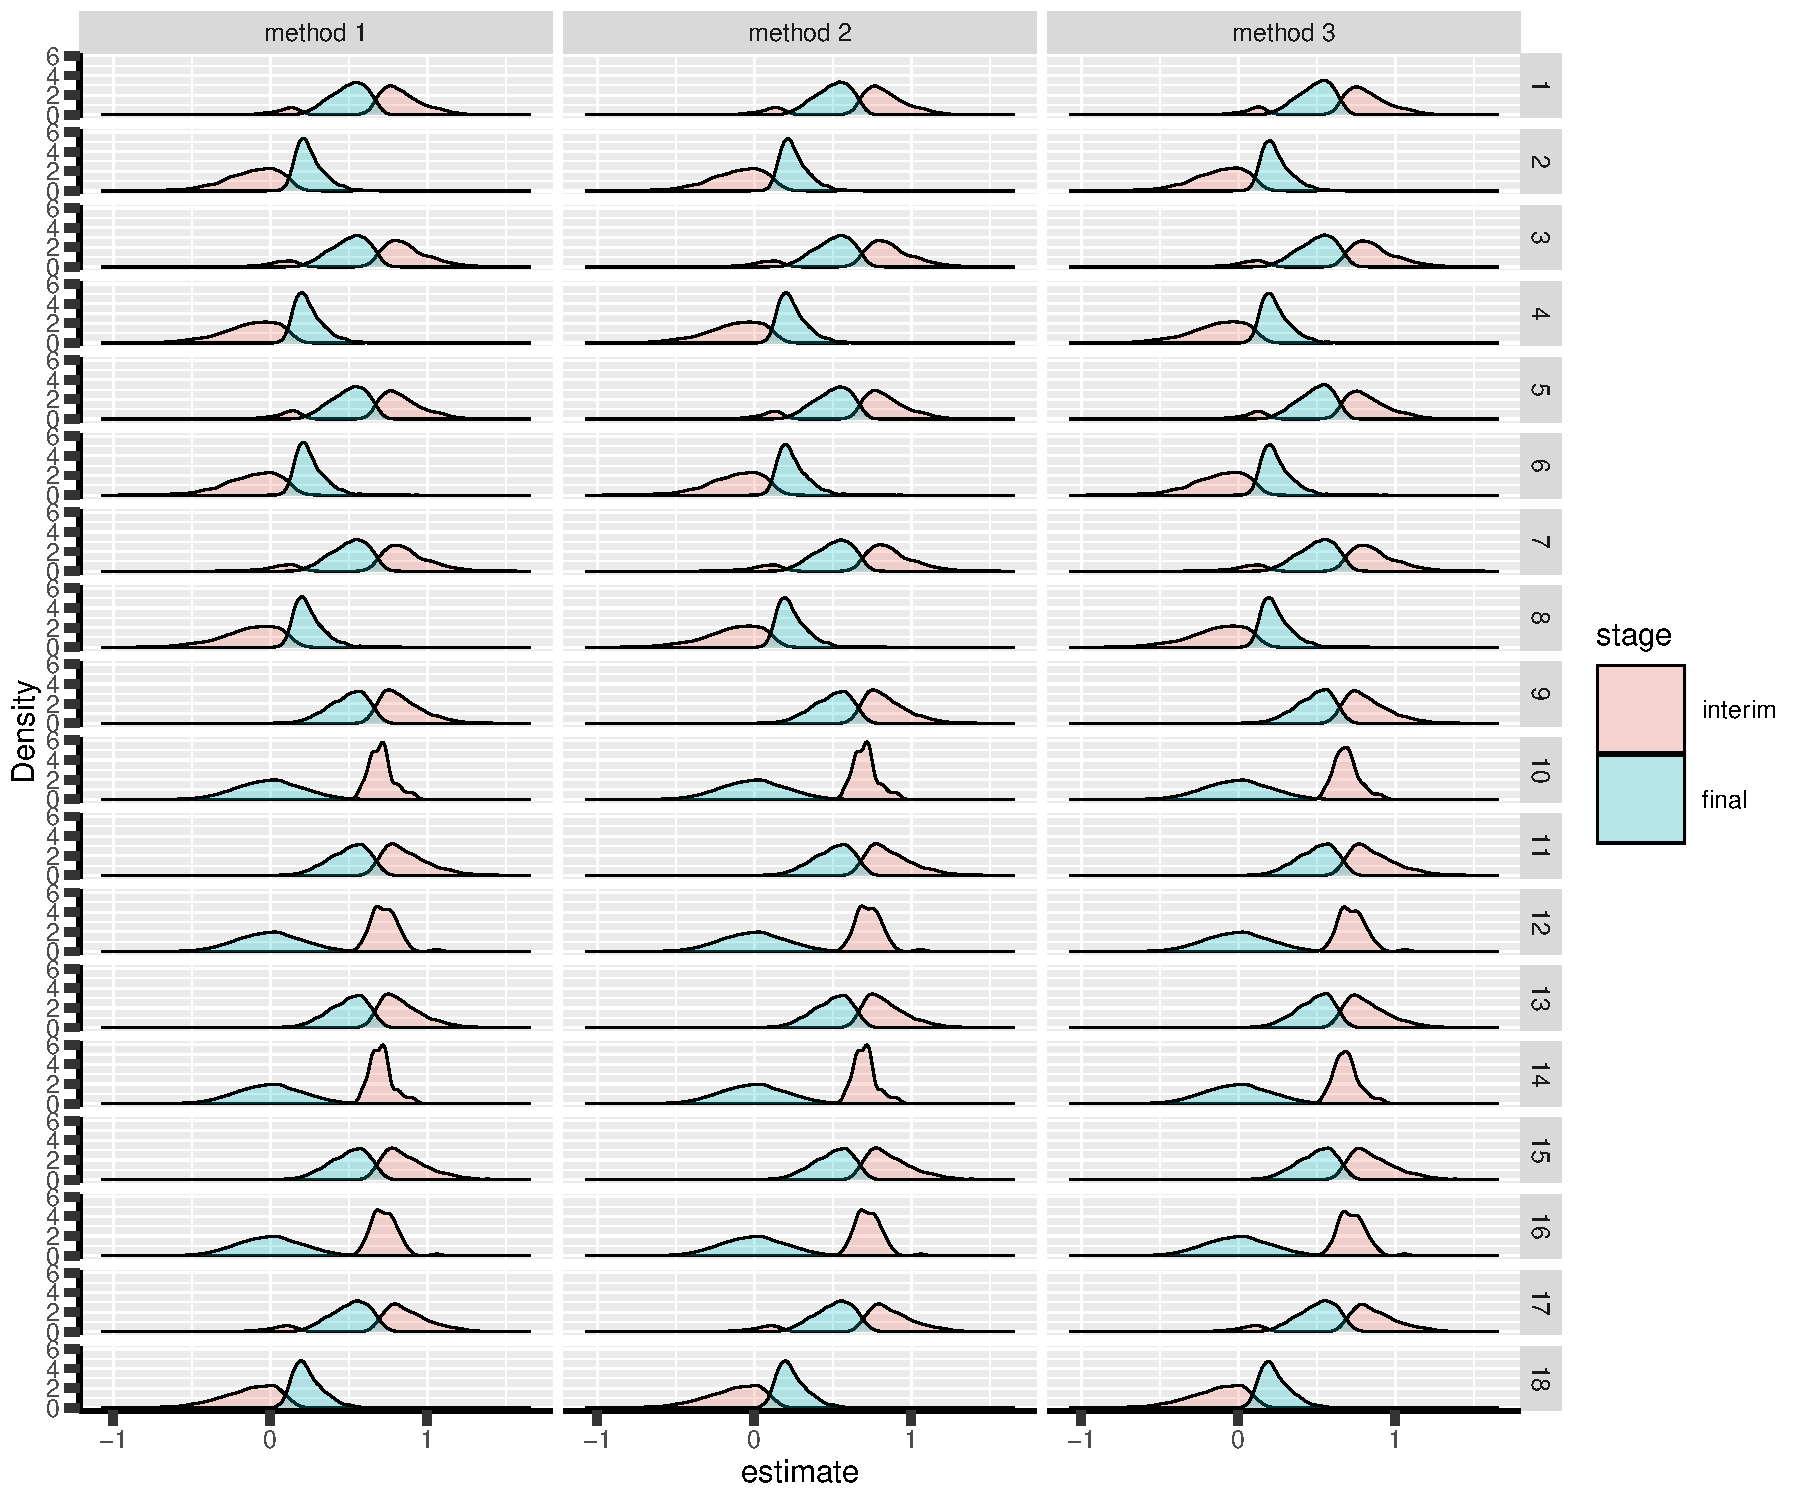
\includegraphics[trim={0 0 0 0},width=1\textwidth]{./figures/gg2stage-estimateC-density.pdf}
\caption{Median unbiased estimate distribution conditional to the stage. Each row correspond to a different scenario.}
\end{figure}

\clearpage

\subsection{3 stages}
\label{sec:org627302a}

Distribution of the estimates:
\begin{figure}[!h]
\centering
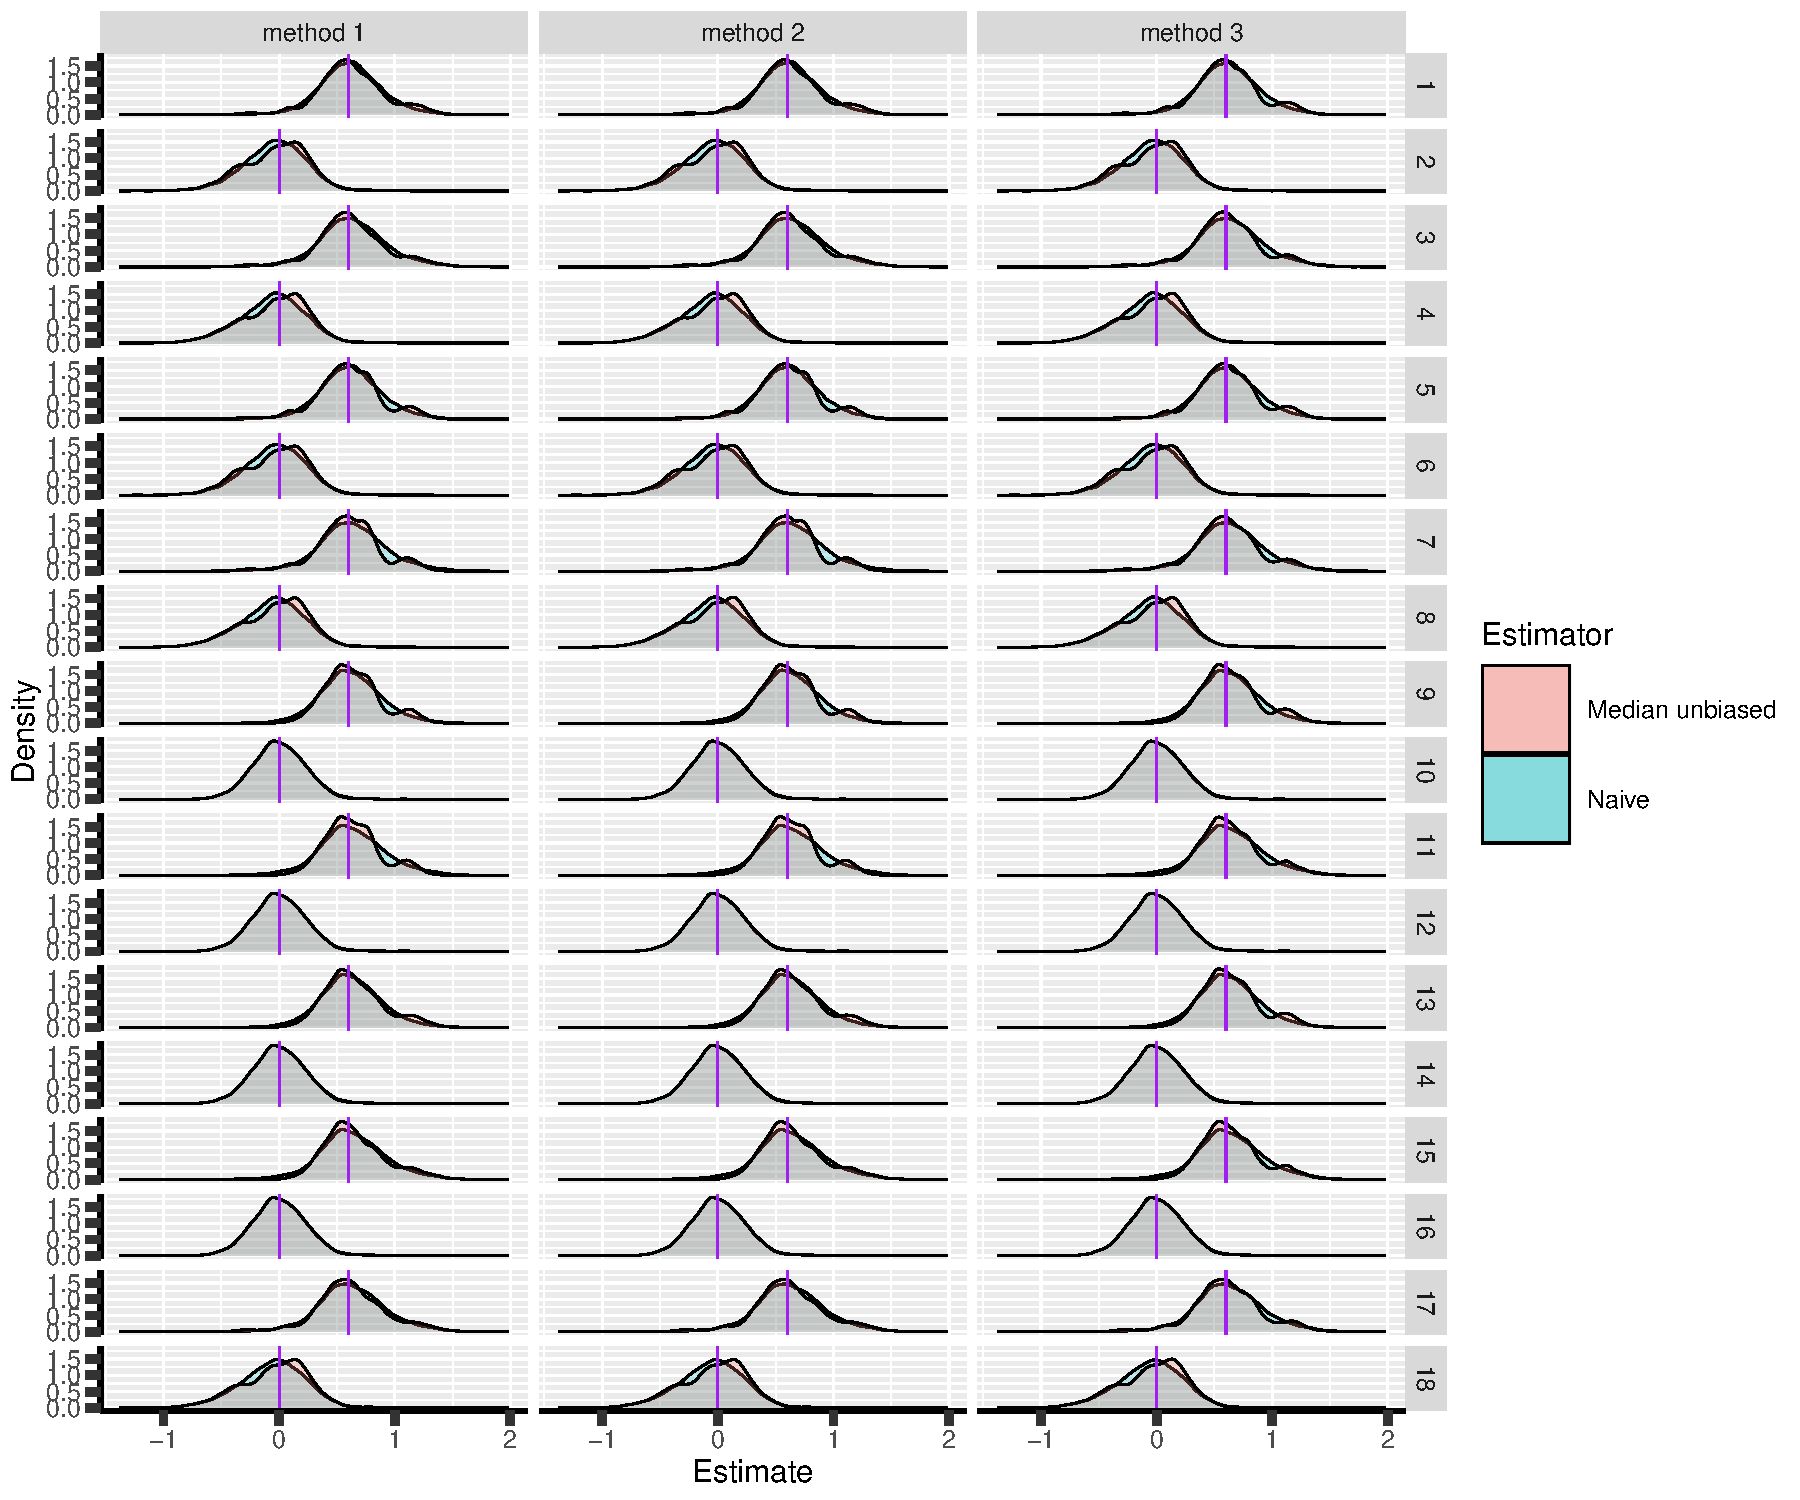
\includegraphics[trim={0 0 0 0},width=1\textwidth]{./figures/gg3stage-estimate-density.pdf}
\caption{Naive and Median unbiased estimate distribution over all simulations. Each row correspond to a different scenario}
\end{figure}

\begin{figure}[!h]
\centering
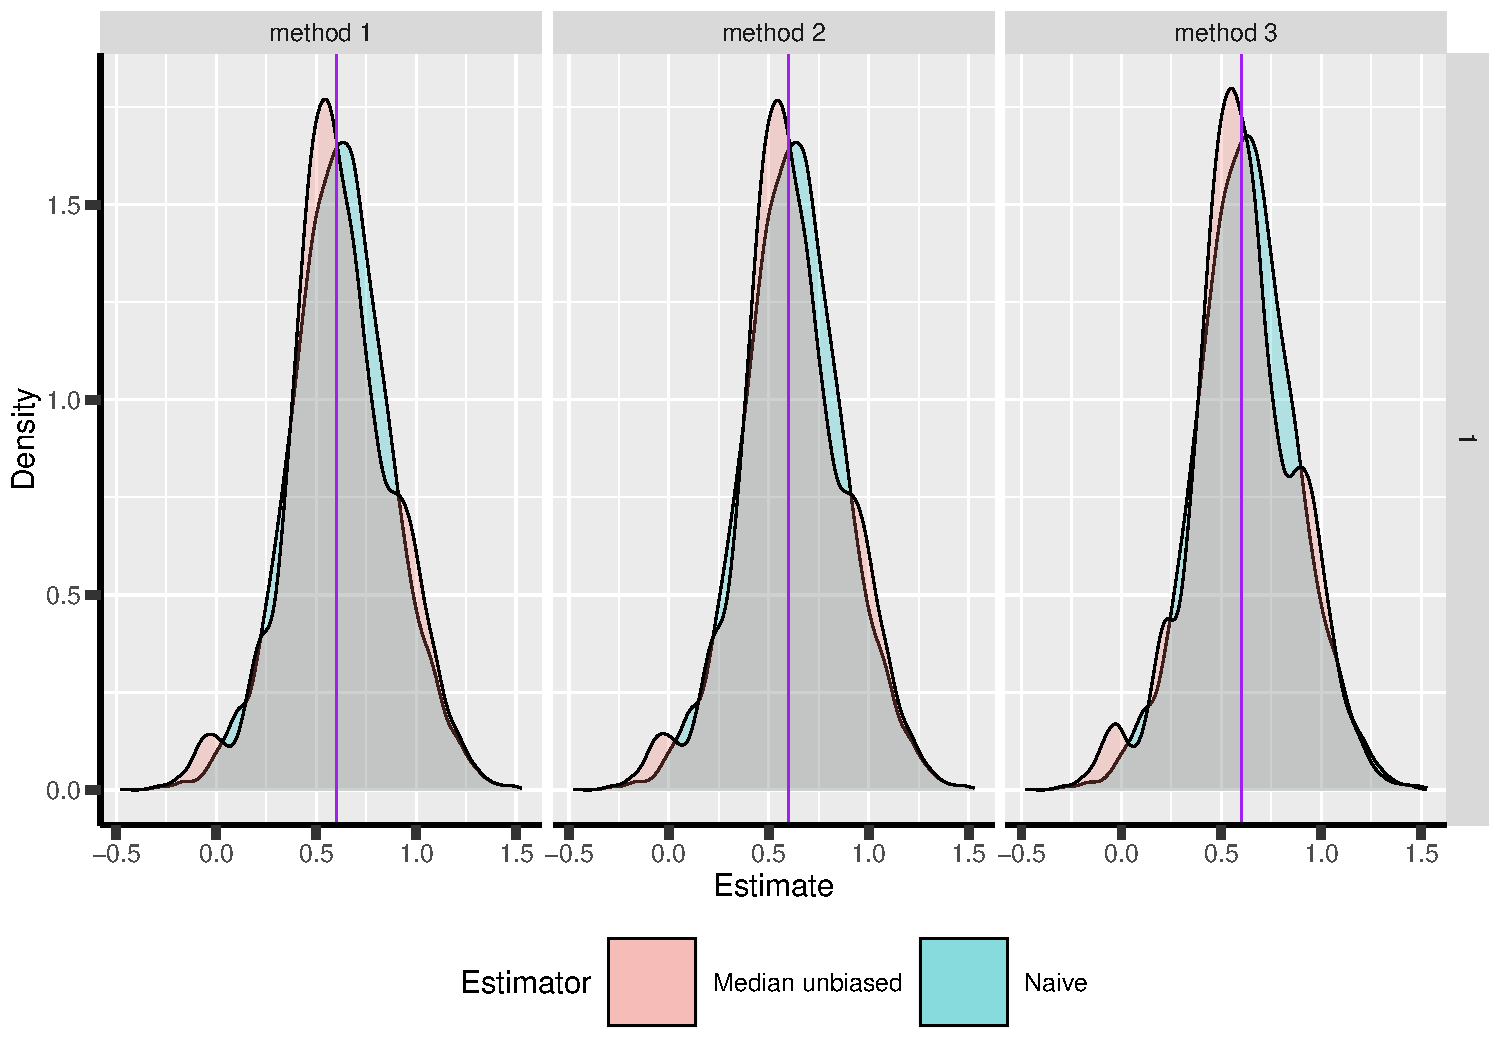
\includegraphics[trim={0 0 0 0},width=\textwidth]{./figures/gg3stage-estimate-density-scenario1.pdf}
\caption{Same but specific to scenario 1}
\end{figure}

\clearpage

Distribution of the median unbiased estimate conditional to the stage:
\begin{figure}[!h]
\centering
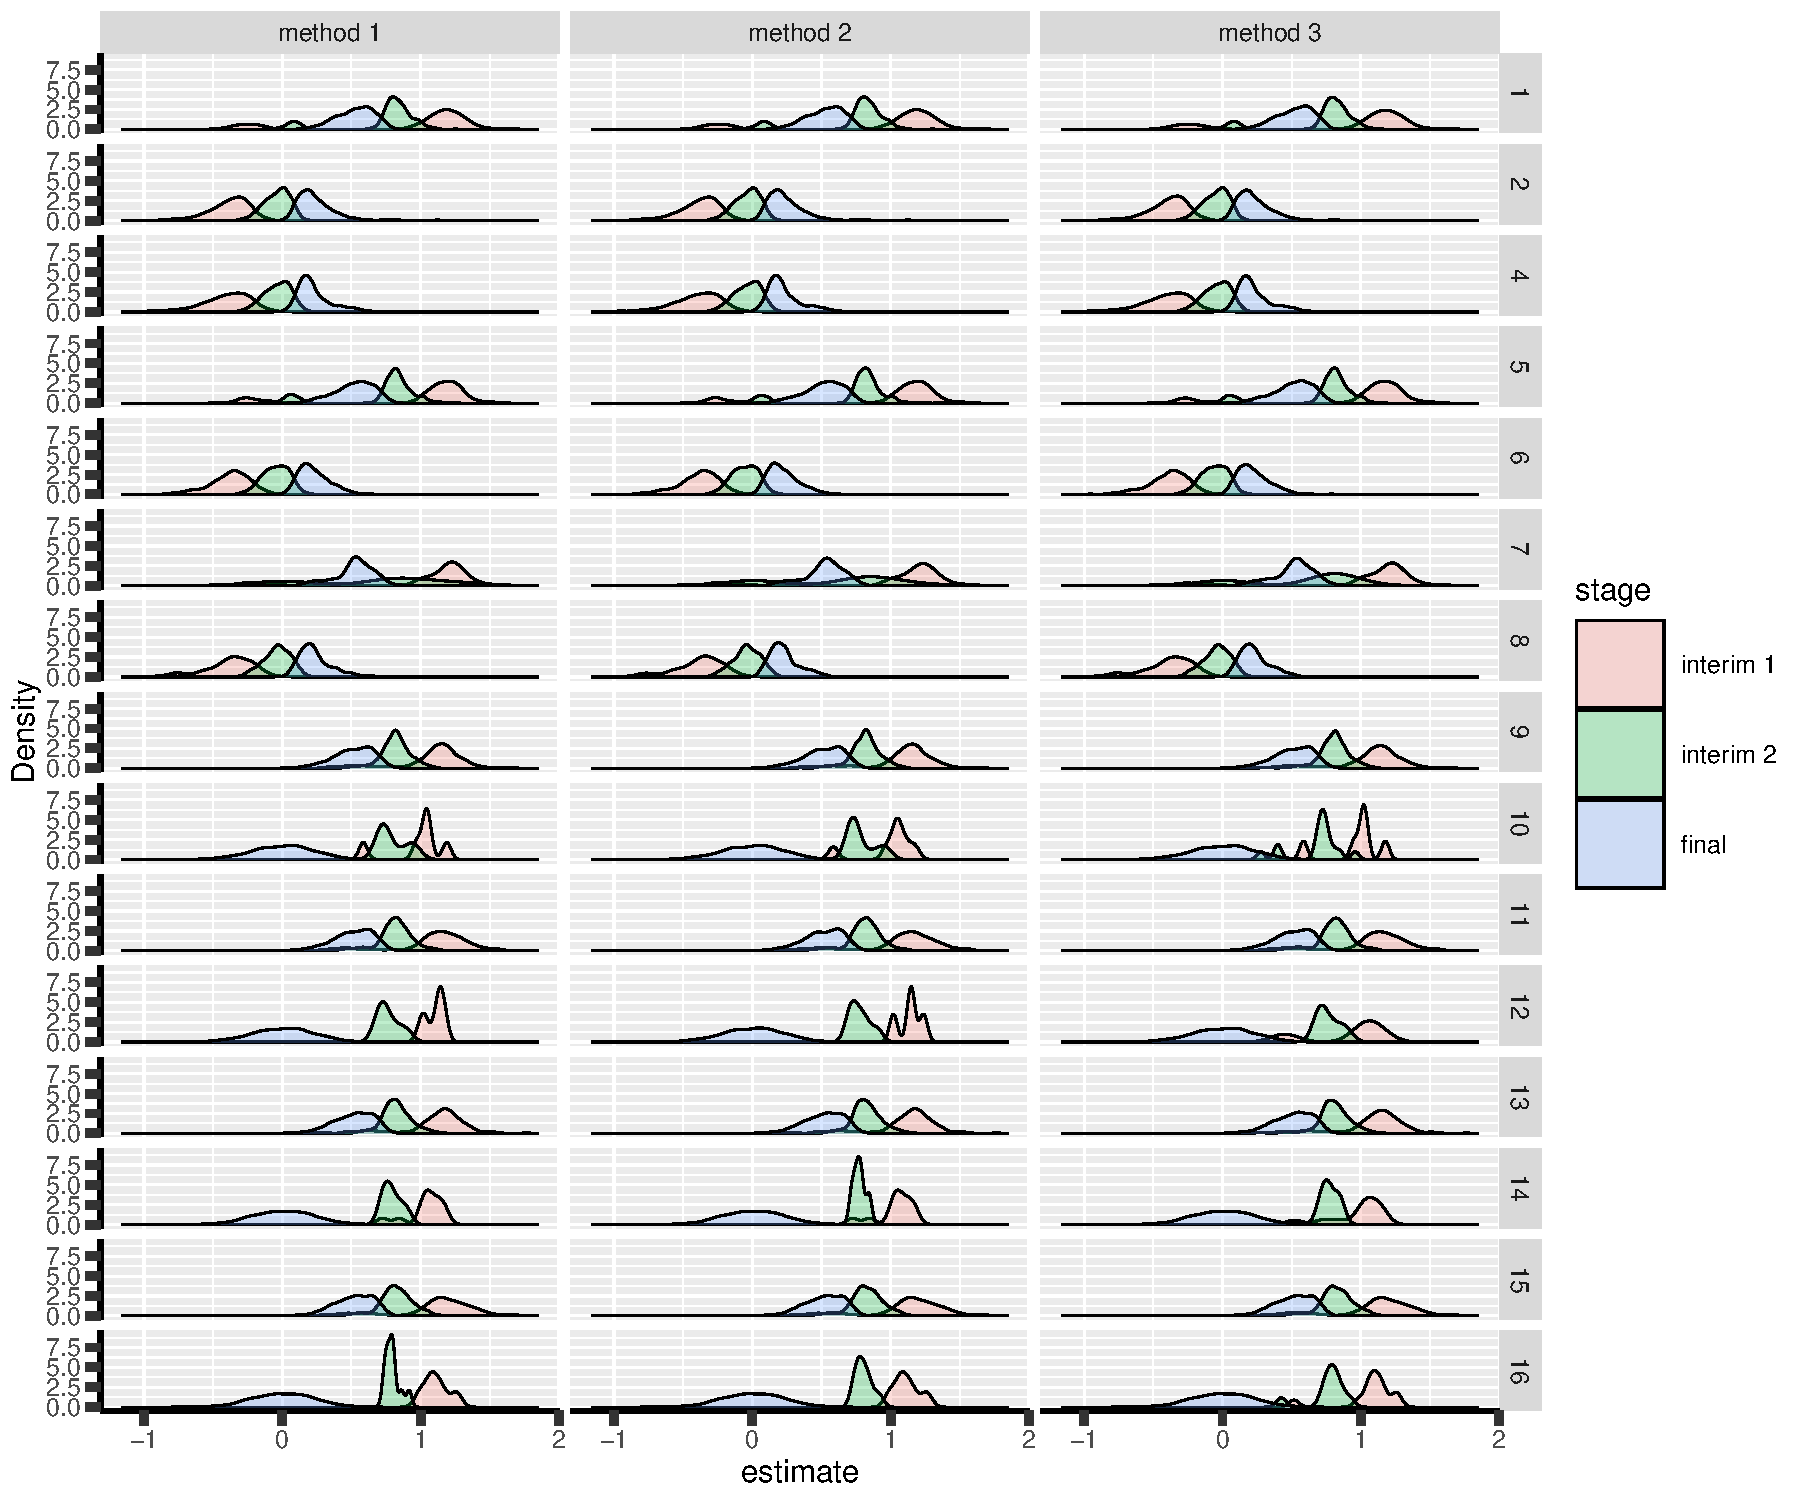
\includegraphics[trim={0 0 0 0},width=1\textwidth]{./figures/gg3stage-estimateC-density.pdf}
\caption{Median unbiased estimate distribution conditional to the stage. Each row correspond to a different scenario.}
\end{figure}

\clearpage

\section{Special cases}
\label{sec:org7094af2}

\subsection{2 stages}
\label{sec:org769a6b0}

Reason for stopping (efficacy, futility, Imax reached), continuing the
trial (decreasing information, no boundary crossed), or concluding
(stop for futility at interim):
\begin{verbatim}
                                    scenario    1    2    3    4    5    6    7    8
reason                       method                                                 
decreasing information       1                  0    0    1    1    0    0    1    1
                             2                  0    0    1    1    0    0    1    1
                             3                  0    0    1    1    0    0    1    1
efficacy                     1               3739   81 3573   74 3739   81 3573   74
                             2               3744   81 3576   74 3718   79 3545   71
                             3               4165  108 3721   82 4165  108 3721   82
futility                     1                632 7111  599 6932  632 7111  599 6932
                             2                659 7161  600 6938  574 6940  562 6828
                             3                545 6844  563 6828  545 6844  563 6828
Imax reached                 1                  1    1    0    0    1    1    0    0
                             2                  1    1    0    0    1    1    0    0
                             3                  1    1    0    0    1    1    0    0
no boundary crossed          1               5628 2807 5828 2994 5628 2807 5828 2994
                             2               5596 2757 5824 2988 5707 2980 5893 3101
                             3               5289 3047 5716 3090 5289 3047 5716 3090
stop for futility at interim 1                  0    0    0    0    0    0    0    0
                             2                  0    0    0    0    0    0    0    0
                             3                 11    1    2    0   11    1    2    0
\end{verbatim}

\begin{verbatim}
                                    scenario    9   10   11   12   13   14   15   16   17   18
reason                       method                                                           
efficacy                     1               3849   81 3680   76 3849   81 3680   76 3396   74
                             2               3829   80 3661   75 3850   81 3683   76 3400   74
                             3               4238  110 3831   82 4238  110 3831   82 3528   80
futility                     1                613 7122  570 6945  613 7122  570 6945  535 6748
                             2                560 6975  541 6838  629 7164  574 6950  539 6755
                             3                516 6890  543 6842  516 6890  543 6842  496 6642
no boundary crossed          1               5538 2797 5750 2979 5538 2797 5750 2979 6069 3178
                             2               5611 2945 5798 3087 5521 2755 5743 2974 6061 3171
                             3               5246 3000 5626 3076 5246 3000 5626 3076 5976 3278
stop for futility at interim 1                  0    0    0    0    0    0    0    0    0    0
                             2                  0    0    0    0    0    0    0    0    0    0
                             3                  8    0    0    0    8    0    0    0    1    0
\end{verbatim}

\clearpage

\subsection{3 stages}
\label{sec:orga3c3574}

Reason for stopping (efficacy, futility, Imax reached), continuing the
trial (decreasing information, no boundary crossed), or concluding
(stop for futility at interim):
\begin{verbatim}
                                    scenario    1    2    4    5    6    7    8
reason                       method                                            
efficacy                     1                529   20    9  566   10   69    5
                             2                529   20    9  584   12   67    7
                             3                566   22    9  609   12   71    5
futility                     1                104 1556  747   98 1501   19  669
                             2                104 1558  747   91 1464   20  663
                             3                 94 1519  739   87 1461   19  665
no boundary crossed          1               2904 2717 1152 2991 2723  362 1122
                             2               2904 2714 1151 2979 2778  364 1131
                             3               2868 2785 1163 2952 2788  359 1130
stop for futility at interim 1                  0    0    0    0    0    0    0
                             2                  0    0    0    0    0    0    0
                             3                  2    1    0    0    0    0    0
\end{verbatim}

\begin{verbatim}
                           scenario    9   10   11   12   13   14   15   16
reason              method                                                 
efficacy            1                782   20  794   16  749   18  764   21
                    2                792   20  798   17  750   17  758   19
                    3                814   21  802   16  804   18  770   21
futility            1                131 2200  118 2242  128 2248  134 2282
                    2                121 2148  120 2242  125 2243  127 2278
                    3                119 2110  119 2216  118 2181  122 2257
no boundary crossed 1               3794 2774 3785 2739 3852 2688 3809 2686
                    2               3795 2825 3773 2737 3854 2694 3822 2692
                    3               3762 2863 3768 2764 3777 2755 3813 2710
\end{verbatim}

\clearpage

\section{Reversal probability}
\label{sec:orgdf46b2f}

\subsection{2 stages}
\label{sec:org13888a5}

Percentage of time we observe a reversal:

\begin{verbatim}
        N  hypo missing ar binding  fixC fu2eff_1 fu2eff_2 fu2eff_3 eff2fu_1 eff2fu_2 eff2fu_3
 1: 10000 power    TRUE 10    TRUE FALSE    0.57%    0.61%        0    0.17%    0.20%    1.07%
 2: 10000 typeI    TRUE 10    TRUE FALSE    0.10%    0.09%        0    0.11%    0.11%    0.34%
 3: 10000 power    TRUE  5    TRUE FALSE    0.08%    0.08%        0    0.07%    0.07%    0.67%
 4: 10000 typeI    TRUE  5    TRUE FALSE    0.02%    0.02%        0    0.02%    0.02%    0.13%
 5: 10000 power    TRUE 10    TRUE  TRUE    0.22%    0.16%        0    0.67%    0.65%    1.07%
 6: 10000 typeI    TRUE 10    TRUE  TRUE    0.02%    0.01%        0    0.21%    0.21%    0.34%
 7: 10000 power    TRUE  5    TRUE  TRUE    0.02%    0.02%        0    0.46%    0.45%    0.67%
 8: 10000 typeI    TRUE  5    TRUE  TRUE        0        0        0    0.08%    0.08%    0.13%
 9: 10000 power    TRUE 10   FALSE  TRUE    0.14%    0.11%        0    0.58%    0.55%    1.04%
10: 10000 typeI    TRUE 10   FALSE  TRUE        0        0        0    0.20%    0.19%    0.33%
11: 10000 power    TRUE  5   FALSE  TRUE    0.01%    0.01%        0    0.46%    0.44%    0.60%
12: 10000 typeI    TRUE  5   FALSE  TRUE        0        0        0    0.06%    0.06%    0.09%
13: 10000 power    TRUE 10   FALSE FALSE    0.41%    0.42%        0    0.21%    0.22%    1.04%
14: 10000 typeI    TRUE 10   FALSE FALSE        0        0        0    0.12%    0.12%    0.33%
15: 10000 power    TRUE  5   FALSE FALSE    0.03%    0.03%        0    0.04%    0.04%    0.60%
16: 10000 typeI    TRUE  5   FALSE FALSE        0        0        0    0.01%    0.01%    0.09%
17: 10000 power   FALSE  5    TRUE FALSE    0.06%    0.07%        0    0.04%    0.04%    0.63%
18: 10000 typeI   FALSE  5    TRUE FALSE    0.01%    0.01%        0    0.01%    0.01%    0.12%
\end{verbatim}

\clearpage

\subsection{3 stages}
\label{sec:org0cd38dc}
Percentage of time we observe a reversal:
\begin{verbatim}
       N  hypo missing ar binding  fixC fu2eff_1 fu2eff_2 fu2eff_3 eff2fu_1 eff2fu_2 eff2fu_3
 1: 1868 power    TRUE 10    TRUE FALSE    0.32%    0.32%        0    0.05%    0.05%    0.59%
 2: 2481 typeI    TRUE 10    TRUE FALSE    0.20%    0.20%        0    0.08%    0.08%    0.16%
 3: 1127 typeI    TRUE  5    TRUE FALSE        0        0        0    0.09%    0.09%    0.18%
 4: 1934 power    TRUE 10    TRUE  TRUE        0        0        0    0.31%    0.31%    0.52%
 5: 2432 typeI    TRUE 10    TRUE  TRUE        0        0        0    0.16%    0.21%    0.21%
 6:  245 power    TRUE  5    TRUE  TRUE        0        0        0    0.41%    0.41%    0.41%
 7: 1042 typeI    TRUE  5    TRUE  TRUE        0        0        0    0.29%    0.38%    0.29%
 8: 2500 power    TRUE 10   FALSE  TRUE    0.04%        0        0    0.28%    0.32%    0.36%
 9: 2500 typeI    TRUE 10   FALSE  TRUE        0        0        0    0.16%    0.12%    0.20%
10: 2500 power    TRUE  5   FALSE  TRUE        0        0        0    0.40%    0.24%    0.40%
11: 2500 typeI    TRUE  5   FALSE  TRUE        0        0        0    0.04%    0.08%    0.04%
12: 2500 power    TRUE 10   FALSE FALSE    0.12%    0.12%        0    0.04%    0.04%    0.44%
13: 2483 typeI    TRUE 10   FALSE FALSE        0        0        0    0.16%    0.12%    0.20%
14: 2500 power    TRUE  5   FALSE FALSE        0        0        0        0        0    0.16%
15: 2500 typeI    TRUE  5   FALSE FALSE        0        0        0        0        0    0.08%
\end{verbatim}


\clearpage

\section{Logical consistency of p-values/CIs}
\label{sec:orgab7644f}


\subsection{Mismatch p-value / boundaries}
\label{sec:orgf13b1c3}
\subsubsection{2 stages}
\label{sec:org9ea0e19}

When concluding for futility:
\begin{verbatim}
     hypo missing ar binding  fixC method 1 method 2 method 3
 1: power    TRUE 10    TRUE FALSE        0        0        0
 2: typeI    TRUE 10    TRUE FALSE        0        0        0
 3: power    TRUE  5    TRUE FALSE        0        0        0
 4: typeI    TRUE  5    TRUE FALSE        0        0        0
 5: power    TRUE 10    TRUE  TRUE        0        0        0
 6: typeI    TRUE 10    TRUE  TRUE        0        0        0
 7: power    TRUE  5    TRUE  TRUE        0        0        0
 8: typeI    TRUE  5    TRUE  TRUE        0        0        0
 9: power    TRUE 10   FALSE  TRUE        0        0        0
10: typeI    TRUE 10   FALSE  TRUE        0        0        0
11: power    TRUE  5   FALSE  TRUE        0        0        0
12: typeI    TRUE  5   FALSE  TRUE        0        0        0
13: power    TRUE 10   FALSE FALSE        0        0        0
14: typeI    TRUE 10   FALSE FALSE        0        0        0
15: power    TRUE  5   FALSE FALSE        0        0        0
16: typeI    TRUE  5   FALSE FALSE        0        0        0
17: power   FALSE  5    TRUE FALSE        0        0        0
18: typeI   FALSE  5    TRUE FALSE        0        0        0
\end{verbatim}

When concluding for efficacy:
\begin{verbatim}
     hypo missing ar binding  fixC method 1 method 2 method 3
 1: power    TRUE 10    TRUE FALSE        0        0        0
 2: typeI    TRUE 10    TRUE FALSE        0        0        0
 3: power    TRUE  5    TRUE FALSE        0        0        0
 4: typeI    TRUE  5    TRUE FALSE        0        0        0
 5: power    TRUE 10    TRUE  TRUE        0        0        0
 6: typeI    TRUE 10    TRUE  TRUE        0        0        0
 7: power    TRUE  5    TRUE  TRUE        0        0        0
 8: typeI    TRUE  5    TRUE  TRUE        0        0        0
 9: power    TRUE 10   FALSE  TRUE        0        0        0
10: typeI    TRUE 10   FALSE  TRUE        0        0        0
11: power    TRUE  5   FALSE  TRUE        0        0        0
12: typeI    TRUE  5   FALSE  TRUE        0        0        0
13: power    TRUE 10   FALSE FALSE        0        0        0
14: typeI    TRUE 10   FALSE FALSE        0        0        0
15: power    TRUE  5   FALSE FALSE        0        0        0
16: typeI    TRUE  5   FALSE FALSE        0        0        0
17: power   FALSE  5    TRUE FALSE        0        0        0
18: typeI   FALSE  5    TRUE FALSE        0        0        0
\end{verbatim}

\clearpage

\subsubsection{3 stages}
\label{sec:org2099d81}

When concluding for futility:
\begin{verbatim}
     hypo missing ar binding  fixC method 1 method 2 method 3
 1: power    TRUE 10    TRUE FALSE        0        0        0
 2: typeI    TRUE 10    TRUE FALSE        0        0        0
 3: typeI    TRUE  5    TRUE FALSE        0        0        0
 4: power    TRUE 10    TRUE  TRUE        0        0        0
 5: typeI    TRUE 10    TRUE  TRUE        0        0        0
 6: power    TRUE  5    TRUE  TRUE        0        0        0
 7: typeI    TRUE  5    TRUE  TRUE        0        0        0
 8: power    TRUE 10   FALSE  TRUE        0    0.16%        0
 9: typeI    TRUE 10   FALSE  TRUE        0        0        0
10: power    TRUE  5   FALSE  TRUE        0        0        0
11: typeI    TRUE  5   FALSE  TRUE        0        0        0
12: power    TRUE 10   FALSE FALSE        0        0        0
13: typeI    TRUE 10   FALSE FALSE        0        0        0
14: power    TRUE  5   FALSE FALSE        0        0        0
15: typeI    TRUE  5   FALSE FALSE        0        0        0
\end{verbatim}

When concluding for efficacy:
\begin{verbatim}
     hypo missing ar binding  fixC method 1 method 2 method 3
 1: power    TRUE 10    TRUE FALSE        0        0        0
 2: typeI    TRUE 10    TRUE FALSE        0        0        0
 3: typeI    TRUE  5    TRUE FALSE        0        0        0
 4: power    TRUE 10    TRUE  TRUE        0        0        0
 5: typeI    TRUE 10    TRUE  TRUE        0        0        0
 6: power    TRUE  5    TRUE  TRUE        0        0        0
 7: typeI    TRUE  5    TRUE  TRUE        0        0        0
 8: power    TRUE 10   FALSE  TRUE        0        0        0
 9: typeI    TRUE 10   FALSE  TRUE        0        0        0
10: power    TRUE  5   FALSE  TRUE        0        0        0
11: typeI    TRUE  5   FALSE  TRUE        0        0        0
12: power    TRUE 10   FALSE FALSE        0    0.05%        0
13: typeI    TRUE 10   FALSE FALSE        0        0        0
14: power    TRUE  5   FALSE FALSE        0    0.05%        0
15: typeI    TRUE  5   FALSE FALSE        0        0        0
\end{verbatim}

\clearpage

\subsection{Mismatch confidence intervals / boundaries}
\label{sec:org48495be}

\subsubsection{2 stages}
\label{sec:orged24ffa}

When concluding for futility:
\begin{verbatim}
     hypo missing ar binding  fixC       method 1       method 2       method 3
 1: power    TRUE 10    TRUE FALSE              0              0  0 (NA: 0.05%)
 2: typeI    TRUE 10    TRUE FALSE              0              0              0
 3: power    TRUE  5    TRUE FALSE              0              0              0
 4: typeI    TRUE  5    TRUE FALSE              0              0              0
 5: power    TRUE 10    TRUE  TRUE              0              0  0 (NA: 0.05%)
 6: typeI    TRUE 10    TRUE  TRUE              0              0              0
 7: power    TRUE  5    TRUE  TRUE              0              0              0
 8: typeI    TRUE  5    TRUE  TRUE              0              0              0
 9: power    TRUE 10   FALSE  TRUE 0 (NA: 32.62%) 0 (NA: 30.38%) 0 (NA: 31.41%)
10: typeI    TRUE 10   FALSE  TRUE  0 (NA: 0.21%)  0 (NA: 0.19%)  0 (NA: 0.34%)
11: power    TRUE  5   FALSE  TRUE 0 (NA: 30.64%) 0 (NA: 29.26%) 0 (NA: 30.24%)
12: typeI    TRUE  5   FALSE  TRUE  0 (NA: 0.06%)  0 (NA: 0.06%)  0 (NA: 0.09%)
13: power    TRUE 10   FALSE FALSE 0 (NA: 30.41%) 0 (NA: 31.13%) 0 (NA: 31.41%)
14: typeI    TRUE 10   FALSE FALSE  0 (NA: 0.12%)  0 (NA: 0.12%)  0 (NA: 0.34%)
15: power    TRUE  5   FALSE FALSE 0 (NA: 29.09%) 0 (NA: 29.28%) 0 (NA: 30.24%)
16: typeI    TRUE  5   FALSE FALSE  0 (NA: 0.01%)  0 (NA: 0.01%)  0 (NA: 0.09%)
17: power   FALSE  5    TRUE FALSE              0              0              0
18: typeI   FALSE  5    TRUE FALSE              0              0              0
\end{verbatim}

When concluding for efficacy:
\begin{verbatim}
     hypo missing ar binding  fixC      method 1      method 2      method 3
 1: power    TRUE 10    TRUE FALSE 0 (NA: 0.02%) 0 (NA: 0.02%) 0 (NA: 0.01%)
 2: typeI    TRUE 10    TRUE FALSE             0             0             0
 3: power    TRUE  5    TRUE FALSE             0             0             0
 4: typeI    TRUE  5    TRUE FALSE             0             0             0
 5: power    TRUE 10    TRUE  TRUE 0 (NA: 0.02%) 0 (NA: 0.02%) 0 (NA: 0.01%)
 6: typeI    TRUE 10    TRUE  TRUE             0             0             0
 7: power    TRUE  5    TRUE  TRUE             0             0             0
 8: typeI    TRUE  5    TRUE  TRUE             0             0             0
 9: power    TRUE 10   FALSE  TRUE 0 (NA: 0.03%) 0 (NA: 0.02%) 0 (NA: 0.01%)
10: typeI    TRUE 10   FALSE  TRUE             0             0             0
11: power    TRUE  5   FALSE  TRUE 0 (NA: 0.01%) 0 (NA: 0.02%) 0 (NA: 0.02%)
12: typeI    TRUE  5   FALSE  TRUE             0             0             0
13: power    TRUE 10   FALSE FALSE 0 (NA: 0.02%) 0 (NA: 0.02%) 0 (NA: 0.01%)
14: typeI    TRUE 10   FALSE FALSE             0             0             0
15: power    TRUE  5   FALSE FALSE 0 (NA: 0.01%) 0 (NA: 0.01%) 0 (NA: 0.02%)
16: typeI    TRUE  5   FALSE FALSE             0             0             0
17: power   FALSE  5    TRUE FALSE 0 (NA: 0.02%) 0 (NA: 0.02%) 0 (NA: 0.03%)
18: typeI   FALSE  5    TRUE FALSE             0             0             0
\end{verbatim}

\subsubsection{3 stages}
\label{sec:org3d53077}

When concluding for futility:
\begin{verbatim}
     hypo missing ar binding  fixC           method 1       method 2           method 3
 1: power    TRUE 10    TRUE FALSE                  0              0                  0
 2: typeI    TRUE 10    TRUE FALSE                  0              0                  0
 3: typeI    TRUE  5    TRUE FALSE                  0              0                  0
 4: power    TRUE 10    TRUE  TRUE                  0              0                  0
 5: typeI    TRUE 10    TRUE  TRUE                  0              0                  0
 6: power    TRUE  5    TRUE  TRUE                  0              0                  0
 7: typeI    TRUE  5    TRUE  TRUE                  0              0                  0
 8: power    TRUE 10   FALSE  TRUE 0.20% (NA: 21.43%) 0 (NA: 20.42%) 1.97% (NA: 18.88%)
 9: typeI    TRUE 10   FALSE  TRUE      0 (NA: 0.12%)  0 (NA: 0.08%)  0.16% (NA: 0.04%)
10: power    TRUE  5   FALSE  TRUE     0 (NA: 19.65%) 0 (NA: 20.36%) 2.51% (NA: 18.33%)
11: typeI    TRUE  5   FALSE  TRUE      0 (NA: 0.04%)  0 (NA: 0.04%)              0.04%
12: power    TRUE 10   FALSE FALSE     0 (NA: 20.39%) 0 (NA: 20.00%) 2.99% (NA: 18.51%)
13: typeI    TRUE 10   FALSE FALSE      0 (NA: 0.17%)  0 (NA: 0.12%)  0.04% (NA: 0.17%)
14: power    TRUE  5   FALSE FALSE     0 (NA: 21.54%) 0 (NA: 20.52%) 0.80% (NA: 19.61%)
15: typeI    TRUE  5   FALSE FALSE                  0              0              0.08%
\end{verbatim}

When concluding for efficacy:
\begin{verbatim}
     hypo missing ar binding  fixC method 1 method 2 method 3
 1: power    TRUE 10    TRUE FALSE        0        0        0
 2: typeI    TRUE 10    TRUE FALSE        0        0        0
 3: typeI    TRUE  5    TRUE FALSE        0        0        0
 4: power    TRUE 10    TRUE  TRUE        0        0        0
 5: typeI    TRUE 10    TRUE  TRUE        0        0        0
 6: power    TRUE  5    TRUE  TRUE        0        0        0
 7: typeI    TRUE  5    TRUE  TRUE        0        0        0
 8: power    TRUE 10   FALSE  TRUE        0        0        0
 9: typeI    TRUE 10   FALSE  TRUE        0        0        0
10: power    TRUE  5   FALSE  TRUE        0        0        0
11: typeI    TRUE  5   FALSE  TRUE        0        0        0
12: power    TRUE 10   FALSE FALSE        0        0        0
13: typeI    TRUE 10   FALSE FALSE        0        0        0
14: power    TRUE  5   FALSE FALSE        0        0        0
15: typeI    TRUE  5   FALSE FALSE        0        0        0
\end{verbatim}

\subsection{Range of p-values}
\label{sec:orgcb7167a}

\subsubsection{2 stages}
\label{sec:orga37518c}
\begin{verbatim}
    missing binding  fixC ar  hypo        method 1        method 2       method 3
 1:    TRUE    TRUE FALSE 10 power      [0;0.9147]      [0;0.9147]     [0;0.9147]
 2:    TRUE    TRUE FALSE 10 typeI  [1e-04;0.9999]  [1e-04;0.9999] [1e-04;0.9999]
 3:    TRUE    TRUE FALSE  5 power      [0;0.9015]      [0;0.9015]     [0;0.9015]
 4:    TRUE    TRUE FALSE  5 typeI  [1e-04;0.9998]  [1e-04;0.9998] [1e-04;0.9998]
 5:    TRUE    TRUE  TRUE 10 power  [7e-04;0.9147]  [7e-04;0.9147]     [0;0.9147]
 6:    TRUE    TRUE  TRUE 10 typeI [0.0016;0.9999] [0.0016;0.9999] [1e-04;0.9999]
 7:    TRUE    TRUE  TRUE  5 power  [1e-04;0.9015]  [1e-04;0.9015]     [0;0.9015]
 8:    TRUE    TRUE  TRUE  5 typeI  [5e-04;0.9998]  [5e-04;0.9998] [1e-04;0.9998]
 9:    TRUE   FALSE  TRUE 10 power       [8e-04;1]       [8e-04;1]          [0;1]
10:    TRUE   FALSE  TRUE 10 typeI      [0.0015;1]      [0.0015;1]      [5e-04;1]
11:    TRUE   FALSE  TRUE  5 power       [1e-04;1]       [1e-04;1]          [0;1]
12:    TRUE   FALSE  TRUE  5 typeI       [6e-04;1]       [5e-04;1]      [2e-04;1]
13:    TRUE   FALSE FALSE 10 power           [0;1]           [0;1]          [0;1]
14:    TRUE   FALSE FALSE 10 typeI       [1e-04;1]       [1e-04;1]      [5e-04;1]
15:    TRUE   FALSE FALSE  5 power           [0;1]           [0;1]          [0;1]
16:    TRUE   FALSE FALSE  5 typeI           [0;1]           [0;1]      [2e-04;1]
17:   FALSE    TRUE FALSE  5 power      [0;0.9642]      [0;0.9642]     [0;0.9642]
18:   FALSE    TRUE FALSE  5 typeI           [0;1]           [0;1]      [3e-04;1]
\end{verbatim}

\clearpage

\subsubsection{3 stages}
\label{sec:orgce511ef}
\begin{verbatim}
    missing binding  fixC ar  hypo        method 1        method 2        method 3
 1:    TRUE    TRUE FALSE 10 power      [0;0.9417]      [0;0.9417]      [0;0.9426]
 2:    TRUE    TRUE FALSE 10 typeI  [1e-04;0.9998]  [1e-04;0.9998]  [4e-04;0.9998]
 3:    TRUE    TRUE FALSE  5 typeI  [1e-04;0.9998]  [1e-04;0.9998]  [3e-04;0.9998]
 4:    TRUE    TRUE  TRUE 10 power  [3e-04;0.9071]  [3e-04;0.8993]  [1e-04;0.9091]
 5:    TRUE    TRUE  TRUE 10 typeI [0.0013;0.9995] [0.0014;0.9995] [0.0012;0.9995]
 6:    TRUE    TRUE  TRUE  5 power  [1e-04;0.8871]  [1e-04;0.8987]      [0;0.8873]
 7:    TRUE    TRUE  TRUE  5 typeI  [9e-04;0.9975]  [9e-04;0.9979]  [9e-04;0.9975]
 8:    TRUE   FALSE  TRUE 10 power       [3e-04;1]       [2e-04;1]           [0;1]
 9:    TRUE   FALSE  TRUE 10 typeI       [8e-04;1]       [8e-04;1]       [7e-04;1]
10:    TRUE   FALSE  TRUE  5 power       [1e-04;1]           [0;1]           [0;1]
11:    TRUE   FALSE  TRUE  5 typeI      [0.0012;1]      [0.0012;1]      [0.0012;1]
12:    TRUE   FALSE FALSE 10 power           [0;1]           [0;1]           [0;1]
13:    TRUE   FALSE FALSE 10 typeI       [7e-04;1]       [7e-04;1]       [8e-04;1]
14:    TRUE   FALSE FALSE  5 power           [0;1]           [0;1]           [0;1]
15:    TRUE   FALSE FALSE  5 typeI  [1e-04;0.9999]  [1e-04;0.9998]  [1e-04;0.9999]
\end{verbatim}

\clearpage 
\section{Coverage}
\label{sec:org3af74a8}

\subsection{2 stages}
\label{sec:org1de7605}
\begin{verbatim}
     hypo missing ar binding  fixC method 1 method 2 method 3
 1: power   FALSE  5    TRUE FALSE 94.79000 94.79000 94.92000
 2: power    TRUE  5   FALSE FALSE 95.86382 95.86207 95.66505
 3: power    TRUE  5   FALSE  TRUE 96.30458 96.26486 95.66505
 4: power    TRUE  5    TRUE FALSE 94.74000 94.74000 94.87000
 5: power    TRUE  5    TRUE  TRUE 95.08000 95.08000 94.87000
 6: power    TRUE 10   FALSE FALSE 95.98172 96.04941 95.75968
 7: power    TRUE 10   FALSE  TRUE 96.79139 96.75297 95.75968
 8: power    TRUE 10    TRUE FALSE 94.84000 94.82000 95.12000
 9: power    TRUE 10    TRUE  TRUE 95.73000 95.65000 95.12000
10: typeI   FALSE  5    TRUE FALSE 95.14000 95.14000 95.15000
11: typeI    TRUE  5   FALSE FALSE 94.86949 94.86949 95.39954
12: typeI    TRUE  5   FALSE  TRUE 94.91695 94.90745 95.39954
13: typeI    TRUE  5    TRUE FALSE 94.82000 94.82000 94.87000
14: typeI    TRUE  5    TRUE  TRUE 94.90000 94.91000 94.87000
15: typeI    TRUE 10   FALSE FALSE 95.01402 95.01402 96.04407
16: typeI    TRUE 10   FALSE  TRUE 95.09116 95.07162 96.04407
17: typeI    TRUE 10    TRUE FALSE 95.16000 95.19000 95.21000
18: typeI    TRUE 10    TRUE  TRUE 95.34000 95.36000 95.21000
\end{verbatim}

Average width of the confidence intervals
\begin{verbatim}
     hypo missing ar binding  fixC  method 1  method 2 method 3
 1: power   FALSE  5    TRUE FALSE 1.0517981 1.0518066 1.053592
 2: power    TRUE  5   FALSE FALSE 1.0355785 1.0355525 1.030753
 3: power    TRUE  5   FALSE  TRUE 1.0410966 1.0414270 1.030753
 4: power    TRUE  5    TRUE FALSE 1.0513207 1.0513607 1.052634
 5: power    TRUE  5    TRUE  TRUE 1.0570088 1.0563598 1.052629
 6: power    TRUE 10   FALSE FALSE 1.0469276 1.0468858 1.039428
 7: power    TRUE 10   FALSE  TRUE 1.0634581 1.0625586 1.039438
 8: power    TRUE 10    TRUE FALSE 1.0624494 1.0626858 1.062576
 9: power    TRUE 10    TRUE  TRUE 1.0765867 1.0753692 1.062555
10: typeI   FALSE  5    TRUE FALSE 1.0431774 1.0431218 1.046821
11: typeI    TRUE  5   FALSE FALSE 0.9997886 0.9998440 1.018905
12: typeI    TRUE  5   FALSE  TRUE 0.9996979 0.9996859 1.018905
13: typeI    TRUE  5    TRUE FALSE 1.0416221 1.0415882 1.045180
14: typeI    TRUE  5    TRUE  TRUE 1.0416986 1.0423673 1.045180
15: typeI    TRUE 10   FALSE FALSE 1.0182710 1.0227130 1.049875
16: typeI    TRUE 10   FALSE  TRUE 1.0183637 1.0101640 1.049882
17: typeI    TRUE 10    TRUE FALSE 1.0459447 1.0453954 1.056218
18: typeI    TRUE 10    TRUE  TRUE 1.0461003 1.0478314 1.056215
\end{verbatim}

Average ratio between the length of the MUE CIs vs. the ML CIs
\begin{verbatim}
     hypo missing ar binding  fixC  method 1  method 2 method 3
 1: power   FALSE  5    TRUE FALSE 1.0554164 1.0554324 1.057018
 2: power    TRUE  5   FALSE FALSE 1.0477000 1.0477317 1.043003
 3: power    TRUE  5   FALSE  TRUE 1.0532445 1.0529897 1.043003
 4: power    TRUE  5    TRUE FALSE 1.0556658 1.0557135 1.056796
 5: power    TRUE  5    TRUE  TRUE 1.0607293 1.0599867 1.056792
 6: power    TRUE 10   FALSE FALSE 1.0539283 1.0540501 1.045799
 7: power    TRUE 10   FALSE  TRUE 1.0695786 1.0683330 1.045809
 8: power    TRUE 10    TRUE FALSE 1.0641965 1.0644562 1.064036
 9: power    TRUE 10    TRUE  TRUE 1.0773006 1.0760174 1.064016
10: typeI   FALSE  5    TRUE FALSE 1.0496649 1.0496083 1.053799
11: typeI    TRUE  5   FALSE FALSE 0.9997633 0.9998237 1.019473
12: typeI    TRUE  5   FALSE  TRUE 0.9998075 0.9997468 1.019473
13: typeI    TRUE  5    TRUE FALSE 1.0486330 1.0486034 1.052752
14: typeI    TRUE  5    TRUE  TRUE 1.0487063 1.0493717 1.052752
15: typeI    TRUE 10   FALSE FALSE 1.0194380 1.0240187 1.051009
16: typeI    TRUE 10   FALSE  TRUE 1.0196328 1.0111242 1.051015
17: typeI    TRUE 10    TRUE FALSE 1.0497075 1.0491459 1.060913
18: typeI    TRUE 10    TRUE  TRUE 1.0498579 1.0516113 1.060910
\end{verbatim}

\clearpage

\section{Percentage of missing values}
\label{sec:orgadf1d47}

At the first interim
\begin{itemize}
\item \texttt{pc.all} percentage of observations with full data (with respect to
all observations, i.e. patients with baseline measurement)
\item \texttt{pc.missing3} percentage of observations missing the final outcome
but with intermediate outcome value and baseline.
\item \texttt{pc.missing23} percentage of observations with only baseline value
\end{itemize}

Here only for method 1 - values are very similar between different
methods:
\begin{verbatim}
    method missing ar  hypo  fixC binding     N   pc.all pc.missing3 pc.missing23
 1:      1    TRUE  5 power FALSE    TRUE 10000 79.52088    9.591086    10.888036
 2:      1    TRUE  5 typeI FALSE    TRUE 10000 79.52088    9.591086    10.888036
 3:      1    TRUE  5 power  TRUE    TRUE 10000 79.52088    9.591086    10.888036
 4:      1    TRUE  5 typeI  TRUE    TRUE 10000 79.52088    9.591086    10.888036
 5:      1    TRUE  5 power  TRUE   FALSE 10000 79.64470    9.441772    10.913523
 6:      1    TRUE  5 typeI  TRUE   FALSE 10000 79.64470    9.441772    10.913523
 7:      1    TRUE  5 power FALSE   FALSE 10000 79.64470    9.441772    10.913523
 8:      1    TRUE  5 typeI FALSE   FALSE 10000 79.64470    9.441772    10.913523
 9:      1   FALSE  5 power FALSE    TRUE 10000 87.78863    6.090240     6.121126
10:      1   FALSE  5 typeI FALSE    TRUE 10000 87.78863    6.090240     6.121126
11:      1    TRUE 10 power FALSE    TRUE 10000 71.59741   13.353880    15.048710
12:      1    TRUE 10 typeI FALSE    TRUE 10000 71.59741   13.353880    15.048710
13:      1    TRUE 10 power  TRUE    TRUE 10000 71.59741   13.353880    15.048710
14:      1    TRUE 10 typeI  TRUE    TRUE 10000 71.59741   13.353880    15.048710
15:      1    TRUE 10 power  TRUE   FALSE 10000 71.79650   13.161615    15.041889
16:      1    TRUE 10 typeI  TRUE   FALSE 10000 71.79650   13.161615    15.041889
17:      1    TRUE 10 power FALSE   FALSE 10000 71.79650   13.161615    15.041889
18:      1    TRUE 10 typeI FALSE   FALSE 10000 71.79650   13.161615    15.041889
\end{verbatim}

\clearpage

\section{Information}
\label{sec:orge03fdcc}

Percentage of information for method 1\footnote{average over the reached stages}:
\begin{verbatim}
 scenario missing binding  fixC ar  interim decision     final
        1    TRUE    TRUE FALSE 10 54.63712 75.34460 102.69691
        2    TRUE    TRUE FALSE 10 54.63712 74.98217 102.36588
        3    TRUE    TRUE FALSE  5 53.26864 64.03618 102.73604
        4    TRUE    TRUE FALSE  5 53.26864 63.58436 102.37416
        5    TRUE    TRUE  TRUE 10 54.63712 75.34460 102.69691
        6    TRUE    TRUE  TRUE 10 54.63712 74.98217 102.36588
        7    TRUE    TRUE  TRUE  5 53.26864 64.03618 102.73604
        8    TRUE    TRUE  TRUE  5 53.26864 63.58436 102.37416
        9    TRUE   FALSE  TRUE 10 54.50012 74.96442 102.53821
       10    TRUE   FALSE  TRUE 10 54.50012 75.17490 103.12700
       11    TRUE   FALSE  TRUE  5 53.15854 63.71662 102.62539
       12    TRUE   FALSE  TRUE  5 53.15854 64.60960 103.12516
       13    TRUE   FALSE FALSE 10 54.50012 74.96442 102.53821
       14    TRUE   FALSE FALSE 10 54.50012 75.17490 103.12700
       15    TRUE   FALSE FALSE  5 53.15854 63.71662 102.62539
       16    TRUE   FALSE FALSE  5 53.15854 64.60960 103.12516
       17   FALSE    TRUE FALSE  5 52.06840 63.77019  99.96969
       18   FALSE    TRUE FALSE  5 52.06840 63.21929  99.62860
\end{verbatim}

Similar results for other methods.
\end{document}